% Emacs settings: -*-mode: latex; TeX-master: "manual.tex"; -*-

\chapter{The component library}
\label{s:components}
This section is devoted to a description of components included in
the component library.  The component library is
maintained by the Ris\o{} group. All components were written at Ris\o\
except the chopper components in
sections~\ref{s:chopper} and~\ref{s:first_chopper} which have been
kindly contributed by Philipp Bernhardt, Lehrstuhl f\"ur
Kristallographie und Strukturphysik; and the Source\_Optimizer
(section~\ref{s:sourceoptimizer}), Monitor\_Optimizer
(section~\ref{s:monitoroptimizer}), and Monitor\_nD
(section~\ref{s:monitornd}) components which were written by Emmanuel
Farhi, Institute Laue-Langevin.
Users are encouraged to send
contributions to us for inclusion in future releases.

In the explanations of the individual components we will use
the usual symbols {\bf r} for the position $(x,y,z)$ of the particle
(unit m), and {\bf v} for 
the particle velocity $(v_x, v_y, v_z)$ (unit m/s).
Another frequently used symbol is 
the wave vector ${\bf k} = m_{\rm N} {\bf v}/\hbar$ , where
$m_{\rm N}$ is the neutron mass. {\bf k} is usually given in
\AA$^{-1}$, while neutron energies are given in meV.
In general, vectors are denoted by boldface symbols.
Subscripts "i" and "f" denotes "initial" and "final", respectively,
and are used in connection with the neutron state before and after
a scattering event.
Note that all mentioning of component geometry refer to
the local coordinate system of the individual component.

The source code for components is listed 
in Appendix~\ref{compcode}. 
The components follow the same numbering
in the Appendix as in the main text, \textit{e.g.} 
component \textbf{Arm}, subsection \ref{explain:arm},
appears in the Appendix as \ref{code:arm}.
Source code for many of the more trivial components are not included in
this manual. All sources may be found in the \verb+lib/mcstas/+
subdirectory of the McStas installation; the default is \verb+/usr/local/lib/mcstas/+.

% Emacs settings: -*-mode: latex; TeX-master: "manual.tex"; -*-

\section{Source components}
The main function of the source components is to determine a set of initial
parameters $({\bf r}, {\bf v})$, or equivalent (${\bf r}, v, \Ombold $),
for each neutron. This is done by Monte Carlo choices. 
In the current sources no polarization dependence is implemented, 
whence we let ${\bf s}=(0,0)$.

The sources to be presented in the following all make their Monte Carlo
choices on the basis of simple analytical expressions ({\em e.g.} the
energy distribution). 
More realistic sources would require that (at least) the Monte-Carlo choice
for the initial energy was made on basis of a measured,
tabulated energy spectrum.
This is planned to be implemented in a later version of \MCS .

\subsection{Source\_flat: A circular continuous source with a flat energy spectrum}
\label{sourceaim}
This component {\bf Source\_flat} is 
a simple continous source with a flat energy distribution.
The time-of-flight aspect is not relevant for this component,
so we put $t=0$ for all neutrons.

The initial neutron position is chosen randomly from within a
circle of radius $r_{\rm s}$ in the $z=0$ plane. 
This is a fair approximation
of a cylindrical cold source with the beam going out along
the cylinder axis, like the one at Ris\o .

The initial neutron velocity direction is focused within
a solid angle, defined by a rectangular target of width
$w$, height $h$, parallel to 
the $xy$ plane placed at $(0,0,z_{\rm f})$. 
A small angle approximation is used, assuming that 
$w,h \ll z_{\rm f}$.

The weight multiplier of the created neutron, $\pi_1$, is set to the
solid angle of the focusing opening divided by $4\pi$,
see discussion in \ref{s:focus}

The input parameters of {\bf Source\_flat} are the source radius, $r_{\rm s}$,
the distance to the target, $z_{\rm f}$, 
the dimensions of the target, $w$ and $h$, and
the centre and spread of the energy distribution, $E_0$ and $\Delta E$.


\subsection{Source\_flat\_lambda: A continous source with flat
  wavelength spectrum}

The component {\bf Source\_flat\_lambda} is similar to the Source\_flat
component, except that the spectrum is flat in wavelength, rather
than in energy.

The input parameters for Source\_flat\_lambda are \textit{radius} to set
the source radius in meters; \textit{dist}, \textit{xw}, and \textit{yh}
to set the focusing as for Source\_flat; and \textit{lambda\_0} and
\textit{d\_lambda} to set the range of wavelength emitted (the range
will be from $\textit{lambda\_0} - \textit{d\_lambda}$ to
$\textit{lambda\_0} + \textit{d\_lambda}$).


\subsection{Source\_flux\_lambda: A continuous source with absolute
  flux}
\label{Source_flux_lambda}

The component {\bf Source\_flux\_lambda} is a variation on the
Source\_flat\_lambda component. The only difference is the possibility
to specify the absolute flux of the source. The specified flux is used
to adjust the initial neutron weight so that the intensity in the
detectors is directly comparable to a measurement of one second on a
real source with the same flux. This also makes the simulated detector
intensities independent of the number of neutron histories simulated,
easing the comparison between different simulation runs (though of
course more neutron histories will give better statistics).

The flux~$\Phi$ is the number of neutrons emitted per second from a
one~cm$^2$ area on the source surface, with direction within a a one
steradian solid angle, and with wavelength within a one {\AA}ngstr{\o}m
interval. The total number of neutrons emitted towards a given diaframe
in one second is therefore
$$ N_{\rm total} = \Phi A \Omega \Delta\lambda $$
where $A$ is the source area, $\Omega$ is the solid angle of the
diaframe as seen from the source surface, and $\Delta\lambda$ is the
width of the wavelength interval in which neutrons are emitted (assuming
a uniform wavelength spectrum). If $N_{\rm sim}$ denotes the number of
neutron histories to simulate, the initial neutron weight $p_0$ must be set to
$$ p_0 = \frac{N_{\rm total}}{N_{\rm sim}} = 
    \frac{\Phi}{N_{\rm sim}} A \Omega \Delta\lambda $$

The input parameters for Source\_flux\_lambda are \textit{radius} to set
the source radius in meters; \textit{dist}, \textit{xw}, and \textit{yh}
to set the focusing as for Source\_flat; \textit{lambda\_0} and
\textit{d\_lambda} to set the range of wavelength emitted (the range
will be from $\textit{lambda\_0} - \textit{d\_lambda}$ to
$\textit{lambda\_0} + \textit{d\_lambda}$); and \textit{flux} to set the
source flux in units of ${\rm cm}^{-2} {\rm st}^{-1} \textit{\AA}$.


\subsection{Source\_div: A divergent source}

{\bf Source\_div} is a rectangular source which emits a
beam of a certain divergence around the main exit direction
(the direction of the $z$ axis).
The beam intensity and divergence are uniform over
the whole of the source, and the energy distribution
of the beam is uniform.

This component may be used as a simple model of the
beam profile at the end of a guide or at the sample
position.

The input parameters for Source\_div are the source dimensions
$w$ and $h$ (in m), the divergencies $\delta_h$ and $\delta_v$ (FWHM in degrees), 
and the mean energy $E_0$ and the energy spread $dE$ (both in meV).
The neutron energy range is $(E_0-dE; E_0+dE)$. 


\subsection{Moderator: A time-of-flight source}
The simple time-of-flight source component {\bf Moderator} resembles
the source component {\bf Source\_flat} described in \ref{sourceaim}.
Like {\bf Source\_flat}, {\bf Moderator} is circular and focuses
on a rectangular target. Further, the initial velocity is chosen
with a linear distribution within an interval, defined by the
minimum and maximum energies, $E_0$ and $E_1$,
respectively.

The initial time of the neutron is determined on basis of a 
simple heuristical model for the time dependence of the 
neutron intensity from a time-of-flight source.
For all neutron energies, the flux decay is assumed to be exponential,
\begin{equation}
\Psi(E,t) = \exp(-t/\tau(E)) ,
\end{equation}
where the decay constant is given by
\begin{equation}
\tau(E) = \left\{ 
\begin{array}{cc}
 \tau_0                               & ; E<E_c \\
 \tau_0 / [ 1 + (E-E_c)^2/\gamma^2 ]  & ; E \geq E_c
\end{array}
\right.
\end{equation}

The input parameters for {\bf Moderator} are the source radius, $r_{\rm s}$,
the minimum and maximum energies, $E_0$ and $E_1$ (in meV),
the distance to the target, $z_{\rm f}$, the dimensions of the target,
$w$ and $h$, and the decay parameters 
$\tau_0$ (in $\mu$s), $E_c$, and $\gamma$ (both in meV).


\section{Source\_adapt: A neutron source with adaptive importance sampling}
\label{s:Source_adapt}
\label{s:source-adapt}
\index{Optimization}
\index{Sources!Adaptive source}

\component{Source\_adapt}{K. Nielsen}{$x_{min}$, $x_{max}$, $y_{min}$, $y_{max}$, $E0$, $dE$, dist, $xw$, $yh$, $\Phi$}{$\alpha$, $\beta$ (plenty, default values are ok)}{partially validated}

{\bf Source\_adapt} is a neutron source that uses adaptive
importance sampling to improve the efficiency of the simulations. It
works by changing on-the-fly the probability distributions from which
the initial neutron state is sampled so that samples in regions that
contribute much to the accuracy of the overall result are preferred over
samples that contribute little. The method can achieve improvements of a
factor of ten or sometimes several hundred in simulations where only a
small part of the initial phase space contains useful neutrons.
This component uses the correlation between neutron energy,
initial direction and initial position.

The physical characteristics of the source are similar to those of
{\bf Source\_simple} (see section~\ref{source-simple}). The source is a thin
rectangle in the $x$-$y$ plane with a flat energy spectrum in a
user-specified range. The flux, $\Phi$, per area per steradian per
{\AA}ngstr{\o}m per second is specified by the user.

The initial neutron weight is given by Eq. (\ref{proprule}) using
$\Delta\lambda$ as the total wavelength range of the source.
A later version of this component will probably include a
$\lambda$-dependence of the flux.

We use the input parameters \textit{dist}, \textit{xw}, and \textit{yh}
to set the focusing as for Source\_simple (section~\ref{source-simple}).
The energy range will be from $E_0 - dE$ to $E_0 + dE$.
\textit{filename} is used to give the name of a file in which to
output the final sampling destribution, see below.
$N_{\rm eng}$, $N_{\rm pos}$, and $N_{\rm div}$
are used to set the number of bins in each dimensions.
Good general-purpose values for the optimization parameters are
$\alpha = \beta = 0.25$. The number of bins to choose will depend on the
application. More bins will allow better adaption of the sampling, but
will require more neutron histories to be simulated before a good
adaption is obtained. The output of the sampling distribution is only
meant for debugging, and the units on the axis are not necessarily
meaningful. Setting the filename to \verb+NULL+ disables the output of
the sampling distribution.

\subsection{Optimization disclaimer}

A warning is in place here regarding potentially wrong results
using optimization techniques.
It is highly recommanded in any case to benchmark 'optimized' simulations
against non-optimized ones, checking that obtained results are the same,
but hopefully with a much improved statistics.

\subsection{The adaption algorithm}

The adaptive importance sampling works by subdividing the initial
neutron phase space into a number of equal-sized bins. The division is
done on the three dimensions of energy, horizontal position, and
horizontal divergence, using $N_{\rm eng}$, $N_{\rm pos}$, and $N_{\rm
  div}$ number of bins in each dimension, respectively. The total number
of bins is therefore
\begin{equation}
N_{\rm bin} = N_{\rm eng} N_{\rm pos} N_{\rm div}
\end{equation}
Each bin $i$ is assigned a sampling weight $w_i$; the probability of
emitting a neutron within bin $i$ is
\begin{equation}
P(i) = \frac{w_i}{\sum_{j=1}^{N_{\rm bin}} w_j}
\end{equation}
In order to avoid false learning, the sampling weight of a bin is
kept larger than $w_{\rm min}$, defined as
\begin{equation}
w_{\rm min} = \frac{\beta}{N_{\rm bin}}\sum_{j=1}^{N_{\rm bin}}w_j,\qquad
    0 \leq \beta \leq 1
\end{equation}
This way a (small) fraction $\beta$ of the neutrons are sampled
uniformly from all bins, while the fraction $(1 - \beta)$ are sampled in an adaptive way.

Compared to a uniform sampling of the phase space (where the probability
of each bin is $1/N_{\rm bin}$), the neutron weight
must be adjusted as given by (\ref{probrule})
\begin{equation}
\pi_1 = \frac{P_1}{f_{\rm MC,1}} =\frac{1/N_{\rm bin}}{P(i)} =
    \frac{\sum_{j=1}^{N_{\rm bin}} w_j}{N_{\rm bin} w_i} ,
\end{equation}
where $P_1$ is understood by the "natural" uniform sampling.

In order to set the criteria for adaption, the {\bf Adapt\_check} component is
used (see section~\ref{s:adapt_check}). The source attemps to sample
only from bins from which neutrons are not absorbed prior to the
position in the instrument at which {\bf Adapt\_check} is
placed. Among those bins, the algorithm attemps to minimize the variance
of the neutron weights at the {\bf Adapt\_check} position. Thus bins that
would give high weights at the {\bf Adapt\_check} position are sampled more
often (lowering the weights), while those with low weights are sampled
less often.

Let $\pi = p_{\rm ac}/p_0$ denote the ratio between the neutron weight $p_1$ at
the {\bf Adapt\_check} position and the initial weight $p_0$ just after the
source. For each bin, the component keeps track of the sum $\Sigma$ of
$\pi$'s as well as of the total number of neutrons $n_i$ from that
bin. The average weight at the {\bf Adapt\_source} position of bin $i$ is thus
$\Sigma_i/n_i$.

We now distribute a total sampling weight of $\beta$ uniformly
among all the bins, and a total weight of $(1 - \beta)$ among bins in
proportion to their average weight $\Sigma_i/n_i$ at the {\bf Adapt\_source}
position:
\begin{equation}
w_i = \frac{\beta}{N_{\rm bin}} +
    (1-\beta) \frac{\Sigma_i/n_i}{\sum_{j=1}^{N_{\rm bins}} \Sigma_j/n_j}
\end{equation}
After each neutron event originating from bin $i$, the sampling weight $w_i$
is updated.

This basic idea can be improved with a small modification. The problem
is that until the source has had the time to learn the right sampling
weights, neutrons may be emitted with high neutron weights (but low
probability). These low probability neutrons may account for a large fraction of
the total intensity in detectors, causing large variances in the
result. To avoid this, the component emits early neutrons with a lower
weight, and later neutrons with a higher weight to compensate. This way
the neutrons that are emitted with the best adaption contribute the most
to the result.

The factor with which the neutron weights are adjusted is given by a
logistic curve
\begin{equation}
  F(j) = C\frac{y_0}{y_0 + (1 - y_0) e^{-r_0 j}}
\end{equation}
where $j$ is the index of the particular neutron history, $1 \leq j
\leq N_{\rm hist}$. The constants $y_0$, $r_0$, and $C$ are given by
\begin{eqnarray}
  y_0 &=& \frac{2}{N_{\rm bin}} \\
  r_0 &=& \frac{1}{\alpha}\frac{1}{N_{\rm hist}}
     \log\left(\frac{1 - y_0}{y_0}\right) \\
  C &=& 1 + \log\left(y_0 + \frac{1 - y_0}{N_{\rm hist}}
     e^{-r_0 N_{\rm hist}}\right)
\end{eqnarray}
The number $\alpha$ is given by the user and specifies (as a fraction
between zero and one) the point at which the adaption is considered
good. The initial fraction $\alpha$ of neutron histories are emitted
with low weight; the rest are emitted with high weight:
\begin{equation}
  p_0(j) =
    \frac{\Phi}{N_{\rm sim}} A \Omega \Delta\lambda
    \frac{\sum_{j=1}^{N_{\rm bin}} w_j}{N_{\rm bin} w_i}
    F(j)
\end{equation}
The choice of the constants $y_0$, $r_0$, and $C$ ensure that
\begin{equation}
\int_{t=0}^{N_{\rm hist}} F(j) = 1
\end{equation}
so that the total intensity over the whole simulation will be correct

Similarly, the adjustment of sampling weights is modified so that the
actual formula used is
\begin{equation}
w_i(j) = \frac{\beta}{N_{\rm bin}} +
    (1-\beta) \frac{y_0}{y_0 + (1 - y_0) e^{-r_0 j}}
     \frac{\psi_i/n_i}{\sum_{j=1}^{N_{\rm bins}} \psi_j/n_j}
\end{equation}

\subsection{The implementation}

The heart of the algorithm is a discrete distribution $p$. The
distribution has $N$ \emph{bins}, $1\ldots N$. Each bin has a value
$v_i$; the probability of bin $i$ is then $v_i/(\sum_{j=1}^N v_j)$.

Two basic operations are possible on the distribution. An \emph{update}
adds a number $a$ to a bin, setting $v_i^{\rm new} = v_i^{\rm old} +
a$. A \emph{search} finds, for given input $b$, the minimum $i$ such
that
\begin{equation}
 b \leq \sum_{j=1}^{i} v_j.
\end{equation}
The search operation is used to sample from the distribution p. If $r$
is a uniformly distributed random number on the interval
$[0;\sum_{j=1}^N v_j]$ then $i = {\rm search}(r)$ is a random number
distributed according to $p$. This is seen from the inequality
\begin{equation}
\sum_{j=1}^{i-1} v_j < r \leq \sum_{j=1}^{i} v_j,
\end{equation}
from which $r \in [\sum_{j=1}^{i-1} v_j; v_i + \sum_{j=1}^{i-1} v_j]$
which is an interval of length $v_i$. Hence the probability of $i$ is
$v_i/(\sum_{j=1}^N v_j)$.
The update operation is used to
adapt the distribution to the problem at hand during a simulation. Both
the update and the add operation can be performed very efficiently.

As an alternative, you may use the {\bf Source\_Optimizer} component
(see section \ref{source-optimizer}).


% Emacs settings: -*-mode: latex; TeX-master: "manual.tex"; -*-

\section{Source\_Optimizer: A general Optimizer for McStas}
\label{s:sourceoptimizer}

This component was contributed by Emmanuel Farhi, Institute
Laue-Langevin.

The component {\bf Source\_Optimizer} optimizes the whole neutron flux
in order to achieve better statistics at each {\bf Monitor\_Optimizer}
location(s) (see section~\ref{s:monitoroptimizer} for this latter
component). It can act on any incoming neutron beam (from any source
type), and more than one optimization criteria location can be placed
along the instrument.

The usage of the optimizer is very simple, and usually does not require
any configuration parameter. Anyway the user can still customize the
optimization {\it via} various {\it options}.

The optimizer efficiency makes it easy to increase the number of events
at optimization criteria locations by a factor of 20, and thus decreases
the signal error bars by a factor 4.5. Higher factors can often be
achieved in practise. Of course, the overall flux remains the same as
without optimizer.

\subsection{The optimization algorithm}

When a neutron reaches the {\bf Monitor\_Optimizer} location(s), the
component records its position ($x$, $y$) and speed ($v_x,
v_y, v_z$) when it passed in the {\bf Source\_Optimizer}. Some
distribution tables of {\it good} neutrons characteristics are then
built.

When a {\it bad} neutron comes to the {\bf Source\_Optimizer} (it would
then have few chances to reach {\bf Monitor\_Optimizer}), it is changed
into a better one. That means that its position and velocity coordinates
are translated to better values according to the {\it good} neutrons
distribution tables. Anyway, the neutron energy ($\surd v_x^2 + v_y^2 +
v_z^2$) is kept as far as possible.

The {\bf Source\_Optimizer} works as follow:
\begin{enumerate}
\item{First of all, the {\bf Source\_Optimizer} determines some limits
    ({\it min} and {\it max}) for variables $x, y, v_x, v_y, v_z$.}
\item{Then the component records the non-optimized flux distributions in
    arrays with {\it bins} cells (default is 10 cells). This constitutes
    the {\it Reference } source.}
\item{\label {SourceOptimizer:step3}The {\bf Monitor\_Optimizer} records
    the {\it good} neutrons (that reach it) and communicate an {\it
      Optimized} source to the {\bf Source\_Optimizer}. However, '{\it
      keep}' percent of the original {\it Reference} source is sent
    unmodified (default is 10 \%). The {\it Optimized} source is thus:

    \begin{center}
      \begin{tabular}{rcl}
        {\it Optimized} & = & {\it keep} * {\it Reference} \\
        & + & (1 - {\it keep}) [Neutrons that will reach monitor].
      \end{tabular}
    \end{center}
    }
\item{The {\bf Source\_Optimizer} transforms the {\it bad} neutrons into
    {\it good} ones from the {\it Optimized} source. The resulting
    optimised flux is normalised to the non-optimized one:
    \begin{equation}
      p_{optimized} = p_{initial} \frac{\mbox{Reference}}{\mbox{Optimized}},
    \end{equation}
    and thus the overall flux at {\bf Monitor\_Optimizer} location is
    the same as without the optimizer. Usually, the process sends more
    {\it good} neutrons from the {\it Optimized} source than than in the
    {\it Reference} one.
    The energy (and velocity) spectra of neutron beam is also kept, as
    far as possible. For instance, an optimization of $v_z$ will induce
    a modification of $v_x$ or $v_y$ to try to keep $|\vec{v}|$
    constant.
    }
\item{When the {\it continuous} optimization option is activated (by
    default), the process loops to Step (\ref{SourceOptimizer:step3})
    every '{\it step}' percent of the simulation. This parameter is
    computed automatically (usually around 10 \%) in {\it auto} mode,
    but can also be set by user.}
\end{enumerate}

During steps (1) and (2), some non-optimized neutrons with original
weight $p_{initial}$ may lead to spikes on detector signals. This is
greatly improved by lowering the weight $p$ during these steps, with the
{\it smooth} option.
The component optimizes the neutron parameters on the basis of
independant variables. Howver, it usually does work fine when these
variables are correlated (which is often the case in the course of the
instrument simulation).
The memory requirements of the component are very low, as no big
$n$-dimensional array is needed.

\subsection{Using the Source\_Optimizer}

To use this component, just install the {\bf Source\_Optimizer} after a
source (but any location is possible in principle), and use the {\bf
  Monitor\_Optimizer} at a location where you want to have better
statistics.

\begin{verbatim}
    /* where to act on neutrons */
    COMPONENT optim_s = Source_Optimizer(options="") 
    ...
    /* where to have better statistics */
    COMPONENT optim_m = Monitor_Optimizer( 
    xmin = -0.05, xmax = 0.05, 
    ymin = -0.05, ymax = 0.05,
    optim_comp = optim_s) 
    ...
    /* using more than one Monitor_Optimizer is possible */
\end{verbatim}

The input parameter for {\bf Source\_Optimizer} is a single {\it
  options} string that can contain some specific optimizer configuration
settings in clear language. The formatting of the {\it options}
parameter is free, as long as it contains some specific keywords, that
can be sometimes followed by values.

The default configuration (equivalent to {\it options} = "") is
\begin{center}
\begin{tabular}{rcl}
  {\it options} & = & "{\it continuous} optimization,
  {\it auto} setting, {\it keep} = 10, {\it bins} = 10, \\
  & & {\it smooth} spikes, and do {\it not free} energy during optimization".
\end{tabular}
\end{center}
The keyword modifiers {\it no} or {\it not} revert the next option.
Other options not shown here are:
\begin{verbatim}
verbose         displays optimization process (debug purpose).
unactivate      to unactivate the Optimizer.
file=[name]     Filename where to save optimized source distributions
\end{verbatim}
The {\it file} option will save the source distributions at the end of
the optimization. If no name is given the component name will be used,
and a '.src' extension will be added. By default, no file is generated.
The file format is in a McStas 2D record style.


% Emacs settings: -*-mode: latex; TeX-master: "manual.tex"; -*-

\section{Simple optical components:
Arms, slits, collimators, filters}
Below we list a number of simple optical components 
which require only a minimum of explanation.

\subsection{Arm: The generic component}
\label{explain:arm}
The component {\bf Arm} is empty; is resembles an optical bench
and has no effect on the neutron.
The function of this component is only to set up a local frame of
reference within the instrument definition. Other components of the
same arm/optical bench may then be
positioned relative to the arm component
using the \MCS\ meta-language.
The use of arm components in the instrument definitions
is not required but is recommended for clarity.

{\bf Arm} has no input parameters.
For more about the use of this component, see the 
sample instrument definitions listed in Appendix \ref{instcode}.


\subsection{Slit: The rectangular slit}
\label{slit}
The component {\bf Slit} is a very simple construction.
It sets up a rectangular opening at $z=0$, and propagates the neutrons 
onto the plane of this rectangle by the kernel call PROP\_Z0.

Neutrons within the slit opening are unaffected, 
while all other neutrons
(no matter how far from the opening their paths intersect the plane)
are discarded by the kernel call ABSORB.
By this simplification, some neutrons contributing to the background
in a real experiment will be neglected. 
These are the ones that scatter off the inner side
of the slit, penetrates the slit material, 
or that clear one of the outer edges of the slit.

The input parameters of {\bf Slit} are the four coordinates,
$(x_{\rm min}, x_{\rm max}, y_{\rm min}, y_{\rm max})$
defining the opening of the rectangle.

\subsection{Circular\_slit: The circular slit}
The component {\bf Circular\_slit} defines a circle in the $z=0$ plane,
centered in the origin. In analogy with {\bf Slit},
neutrons are propagated to this plane, and those which intersect
the plane outside the circle are ABSORB'ed.

The only input parameter of {\bf Circular\_slit} is
the radius, $r$, of the circle.

\subsection{Beamstop\_rectangular: The rectangular beam stop}
\label{s:Beamstop_rectangular}
The component {\bf Beamstop\_rectangular} models a thin, infinitely
absorbing rectangle in the $X$-$Y$ plane, centered on the origin. The
input parameters are \textit{xmin}, \textit{xmax}, \textit{ymin}, and
\textit{ymax} defining the edges of the slit in meters.


\subsection{Beamstop\_circular: The circular beam stop}
\label{s:Beamstop_circular}
The component {\bf Beamstop\_circular} models a thin, infinitely
absorbing circular disk in the $X$-$Y$ plane, centered on the origin. It
takes a single input parameter \textit{radius} to define the circle
radius in meters.


\subsection{Soller: The simple Soller blade collimator}
The component {\bf Soller} defines two rectangular openings
like the one in {\bf Slit}. Neutrons not clearing both these
openings are ABSORB'ed, see the discussion in \ref{slit}.
The collimating effect is taken care of by employing an ideal
triangular transmission through the collimator, as explained below.
For a more detailed Soller collimator simulation the Channeled\_guide
component can be employed, see section~\ref{s:channeled_guide}.

Let the collimation angle be $\delta = \tan^{-1}(d/L)$,
where $L$ is the length of the collimator
and $d$ is the distance between the blades,
and let $\phi$ be the divergence angle between the 
neutron path and a vertical plane along the collimator axis, 
see Fig.~\ref{f:collimator}. Neutrons with a large 
divergence angle $|\phi| \geq \delta$ will always
hit at least one collimator blade and will thus be absorbed.
For smaller divergence angles, $|\phi| < \delta$, the fate of the
neutron depends on its exact entry point.
Assuming that a typical collimator has many blades, the
absolute position of each blade perpendicular to the collimator axis
is somewhat uncertain (and also unimportant).
A simple statistical consideration now shows that the transmission
probability is $T = 1-\tan|\phi|/\tan\delta$.

\begin{figure}
  \begin{center}
    \psfrag{xmin}[c][c]{$x_{\rm min}$}
    \psfrag{xmax}[c][c]{$x_{\rm max}$}
    \psfrag{ymin}[c][c]{$y_{\rm min}$}
    \psfrag{ymax}[c][c]{$y_{\rm max}$}
    \psfrag{delta}[c][c]{$\delta$}
    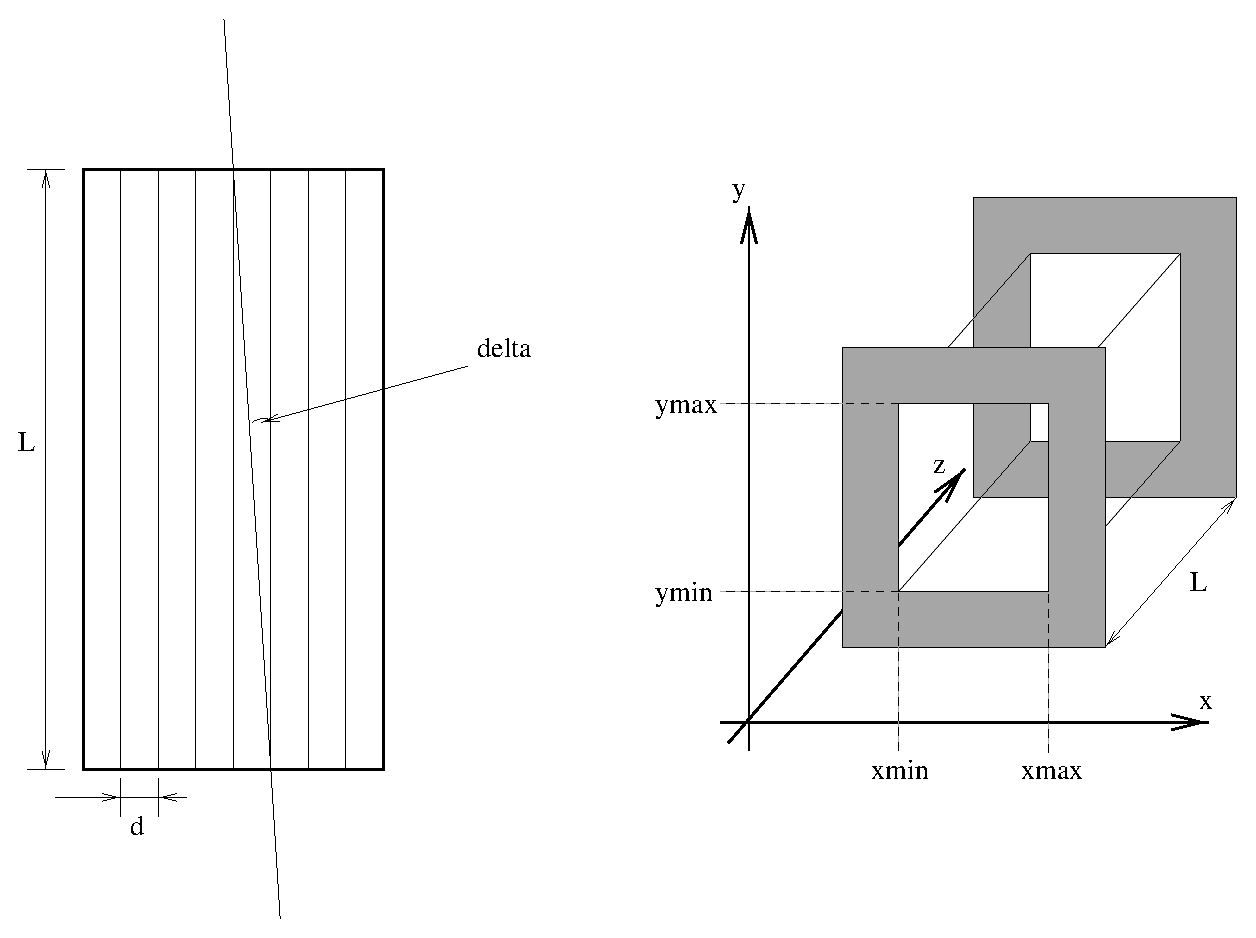
\includegraphics[width=0.9\textwidth]{figures/collimator.eps}
  \end{center}
\caption{The geometry of a simple Soller blade collimators:
The real Soller collimator, seen from the top (left), 
and a sketch of the component {\bf Soller} (right).
The symbols are defined in the text.}
\label{f:collimator}
\end{figure}

We simulate the collimator by transmitting all neutrons with
$|\phi| < \delta$, but adjusting their weight with the amount
\begin{equation}
\pi_i = T = 1-\tan|\phi|/ \tan\delta ,
\end{equation}
while all others are discarded by the kernel call ABSORB.

The input parameters for {\bf Soller} are the coordinates
$(x_{\rm min}, x_{\rm max}, y_{\rm min}, y_{\rm max})$,
defining the identical entry and exit apertures, 
the length, $l$, between the slits, 
and the collimator divergence $\delta$.
If $\delta=0$, the collimating effect is disabled,
so that $\pi_i = 1$ whenever the neutron clears the two apertures.

\subsection{Filter: A transmission filter}
A neutron transmission filter act in much of the same way as two
identical slits, one after the other.
The only difference is that the transmission of the filter
varies with the neutron energy.

In the simple component {\bf Filter},
we have not tried to simulate the details of the transmission
process (which includes absorption, incoherent scattering,
and Bragg scattering in a polycrystalline sample, {\em e.g.} Be).
Instead, the transmission is parametrised to be
$\pi_i=T_0$ when $E \leq E_{\rm min}$, $\pi_i=T_1$ when $E \geq E_{\rm max}$,
and linearly interpolated between the two values
in the intermediate interval.
\begin{equation}
\pi_i = \left\{ \begin{array}{lc}
 T_0  & E \leq E_{\rm min} \\
 T_1 + (T_0-T_1) \frac{E_{\rm max}-E}{E_{\rm max}-E_{\rm min}}
 & E_{\rm min} < E < E_{\rm max} \\
 T_1  & E_\geq E_{\rm max} \\
\end{array} \right.
\end{equation}
If $T_1=0$, the neutrons with $E>E_{\rm max}$ are ABSORB'ed.

The input parameters are the four slit coordinates, 
$(x_{\rm min}, x_{\rm max}, y_{\rm min}, y_{\rm max})$,
the distance, $l$, between the slits, and the transmission parameters 
$T_0$, $T_1$, $E_{\rm min}$, and $E_{\rm max}$. 
The energies are given in meV.


\index{Optics|textbf}

This section describes advanced neutron optical
components such as supermirrors and guides.
A description of the reflectivity of a supermirror is found
in section~\ref{s:mirror}.

\section{Mirror: The single mirror}
\label{s:mirror}
\index{Optics!Mirror plane}
\component{Mirror}{System}{$l$, $h$, $m$}{$R_0, Q_c, W, \alpha$}{validated, no gravitation support}

The component {\bf Mirror}
models a single rectangular neutron mirror plate. It can be used
as a sample component or to \textit{e.g.}~assemble a complete neutron guide by putting multiple
mirror components at appropriate locations and orientations in the
instrument definition, much like a real guide is build from individual
mirrors.

In the local coordinate system, the mirror lies in the first quadrant of the
$x$-$y$ plane, with one corner at $(0,0,0)$.

The input parameters of this component are
the rectangular mirror dimensions $(l, h)$
and the values of $R_0, m, Q_c, W$, and $\alpha$ for the mirror reflectivity.
As a special case, if $m=0$ then the reflectivity is zero for all $Q$,
\textit{i.e.}\ the surface is completely absorbing.

This component may produce wrong results with gravitation.

\subsection{Mirror reflectivity}
\label{ss:mirrorreflect}
To compute the reflectivity of the supermirrors, we use an empirical
formula derived from experimental data \cite{pb_241_50},
see Fig.~\ref{f:reflectivity}. The reflectivity is given by
\begin{equation} \label{e:Rmirror}
  R = \left\{
    \begin{array}{ll}
      R_0 & \textrm{if $Q \leq Q_{\rm c}$} \\
      \frac{1}{2}R_0(1 - \tanh[(Q - m Q_{\rm c})/W])(1-\alpha(Q-Q_{\rm c}))
         & \textrm{if $Q > Q_{\rm c}$}
    \end{array}
  \right.
\end{equation}

Here $Q$ is the length of the scattering vector (in \AA$^{-1}$)
defined by
\begin{equation} \label{e:reflectivity}
Q = |{\bf k}_{\bf i} - {\bf k}_{\bf f}|
  = \frac{m_{\rm n}}{\hbar} |{\bf v}_{\bf i} - {\bf v}_{\bf f}|,
\end{equation}
$m_{\rm n}$ being the neutron mass.
The number $m$ in (\ref{e:Rmirror}) is a parameter determined by
the mirror materials,
the bilayer sequence, and the number of bilayers.
As can be seen, $R=R_0$ for $Q < Q_{\rm c}$, where $Q_{\rm c}$ is the
critical scattering wave vector for a single layer of the mirror
material. At higher values of $Q$, the reflectivity starts falling
linearly with a slope $\alpha$ until a "soft cut-off" at $Q = m Q_{\rm c}$.
The width of this cut-off is denoted $W$. See the example reflection curve in
figure~\ref{f:reflectivity}.

It is {\bf important} to notice that when $m < 1$, the reflectivity remains constant at $R=R_0$ up to $q=Qc$, and \emph{not} $m.Q_c$. This means that $m < 1$ parameters behave like $m=1$ materials.

\subsection{Algorithm}
The function of the component can be described as
\begin{enumerate}
\item Propagate the neutron ray to the plane of the mirror.
\item If the neutron trajectory intersects the mirror plate, it is
reflected, otherwise it is left untouched.
\item Reflection of the incident velocity
${\bf v}_{\rm i} = (v_x,v_y,v_z)$
gives the final velocity ${\bf v}_{\rm f} = (v_x,v_y,-v_z)$.
\item Calculate $Q=2 m_{\rm n} v_z / \hbar$.
\item The neutron weight is adjusted with the amount $\pi_i = R(Q)$.
\item  To avoid spending large amounts of computation time on very low-weight
neutrons, neutrons for which the reflectivity is lower than about
$10^{-10}$ are ABSORB'ed.
\end{enumerate}

\begin{figure}
  \begin{center}
    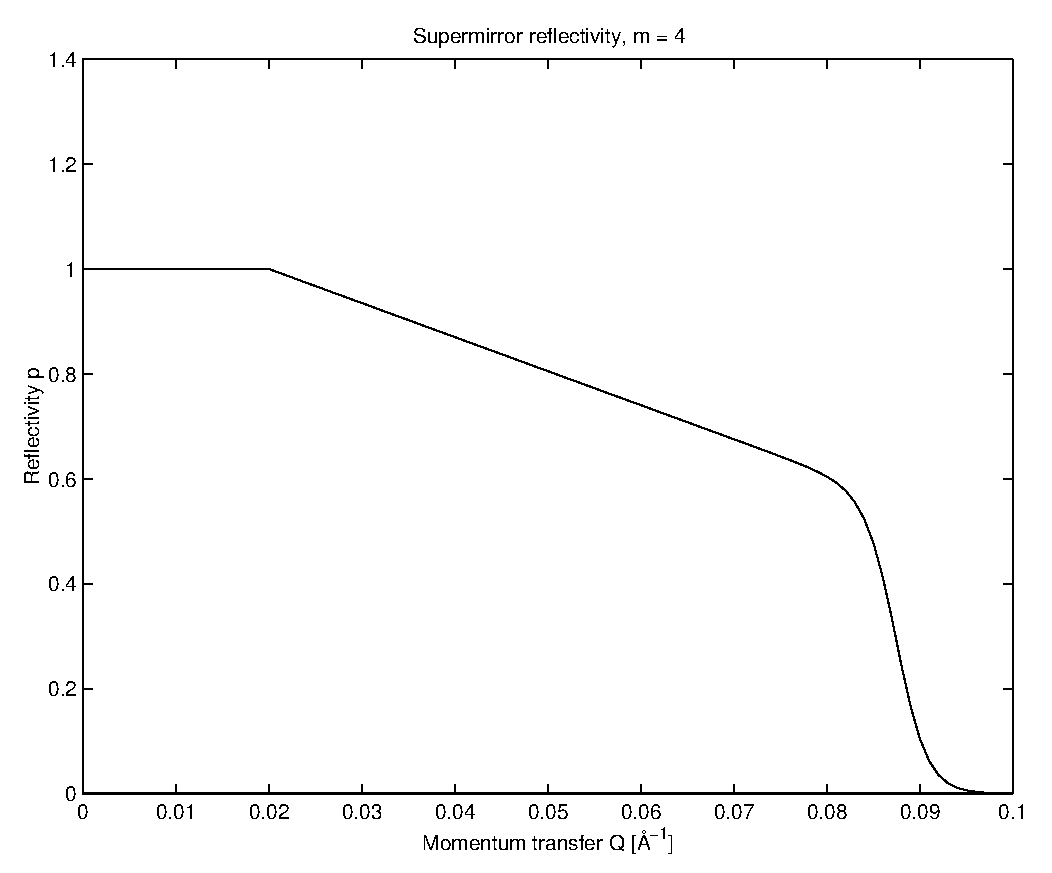
\includegraphics[width=0.6\textwidth]{figures/supermirror.eps}
  \end{center}
\caption{A typical reflectivity curve for a supermirror,
Eq.~(\protect\ref{e:reflectivity}). The used values are
$ m=4$, $R_0=1$, $Q_{\rm c} = 0.02$~\AA$^{-1}$, $\alpha = 6.49$~\AA,
$ W=1/300$~\AA$^{-1}$.
}
\label{f:reflectivity}
\end{figure}

\newpage

\section{Guide: The guide section}
\index{Optics!Straight guide}

\component{Guide}{System}{$w_1, h_1$, $w_2, h_2$, $l$, $m$}{$R_0, Q_c, W, \alpha$}{validated, no gravitation support}

The component {\bf Guide}
models a guide tube consisting of four flat mirrors. The
guide is centered on the $z$ axis with rectangular entrance and exit
openings parallel to the $x$-$y$ plane. The entrance has the dimensions
$(w_1,h_1)$ and placed at $z=0$. The exit is of dimensions $(w_2,h_2)$
and is placed at $z=l$ where $l$ is the guide length. See
figure~\ref{f:guide}.
The reflecting properties are given by the values of
$R_0, m, Q_c, W$, and $\alpha$, as for {\bf Mirror}.

{\bf Guide} may produce wrong results with gravitation support.
Use {\bf Guide\_gravity} (section \ref{s:guide_gravity}) in this case.
For a more general guide simulation, see {\bf Guide\_channeled}
in section~\ref{s:channeled_guide}.

\begin{figure}
  \begin{center}
    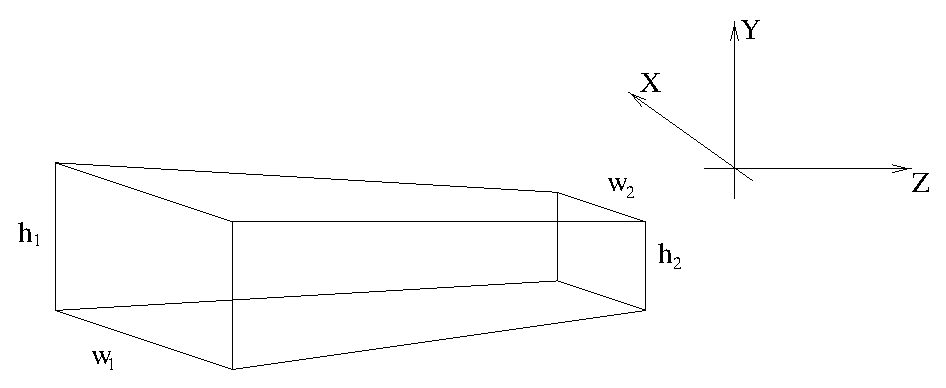
\includegraphics[width=0.7\textwidth]{figures/guide1.eps}
  \end{center}
\caption{The geometry used for the guide component.}
\label{f:guide}
\end{figure}

\subsection{Guide geometry and reflection}
For computations on the guide geometry, we define the planes of the four
guide sides by giving their normal vectors (pointing into the guide)
and a point lying in the plane:
$$
\begin{array}{rclcrcl}
{\bf n}^v_1 &=& (l, 0, {(w_2 - w_1) / 2})
     & & {\bf O}^v_1 &=& (- w_1 / 2, 0, 0) \\
{\bf n}^v_2 &=& (-l, 0, {(w_2 - w_1) / 2})
     & & {\bf O}^v_2 &=& (w_1 / 2, 0, 0) \\
{\bf n}^h_1 &=& (0, l, {(h_2 - h_1) / 2})
     & & {\bf O}^h_1 &=& (0, - h_1 / 2, 0) \\
{\bf n}^h_2 &=& (0, -l, {(h_2 - h_1) / 2})
     & & {\bf O}^h_2 &=& (0, h_1 / 2, 0) \\
\end{array}
$$
In the following, we refer to an arbitrary guide side by its origin
{\bf O} and normal {\bf n}.

With these definitions, the time of intersection of the neutron with a
guide side can be computed by considering the projection onto the
normal:
\begin{equation}
t^\alpha_\beta = \frac{({\bf O}^\alpha_\beta - {\bf r}_0) \cdot {\bf n}^\alpha_\beta}
  {{\bf v} \cdot {\bf n}^\alpha_\beta}  ,
\end{equation}
where $\alpha$ and $\beta$ are indices for the different guide walls,
assuming the values (h,v) and (1,2), respectively.
For a neutron that leaves the guide directly through the guide exit we have
\begin{equation}
t_{\rm exit} = \frac{l - z_0}{v_z}
\end{equation}

The reflected velocity ${\bf v}_{\rm f}$ of the neutron with incoming velocity
${\bf v}_{\rm i}$ is computed by the formula
\begin{equation}
 {\bf v}_{\rm f} =
  {\bf v}_{\rm i}
   - 2{{\bf n} \cdot {\bf v}_{\rm i} \over {|{\bf n}|^2}} {\bf n}
\end{equation}
This expression is arrived at by again considering the projection onto
the mirror normal (see figure~\ref{f:guidereflect}). The reflectivity of the
mirror is taken into account as explained in section~\ref{s:mirror}.

\begin{figure}
  \begin{center}
    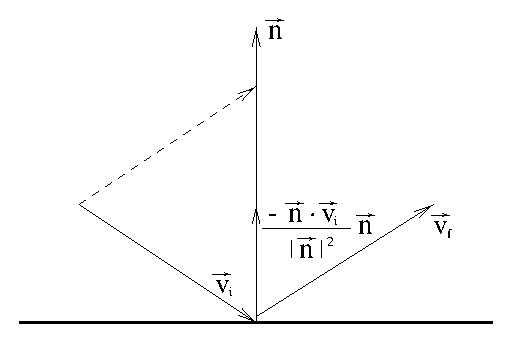
\includegraphics[width=0.5\textwidth]{figures/guide2.eps}
  \end{center}
\caption{Neutron reflecting from mirror. ${\bf v}_{\rm i}$ and
${\bf v}_{\rm f}$ are the initial and final velocities, respectively,
and {\bf n} is a vector normal to the mirror surface.}
\label{f:guidereflect}
\end{figure}

\subsection{Algorithm}
\begin{enumerate}
\item The neutron is initially propagated to the $z = 0$ plane of the
guide entrance.
\item If it misses the entrance, it is ABSORB'ed.
\item Otherwise, repeatedly compute the time of intersection with the
four mirror sides and the guide exit.
\item The smallest positive $t$ thus
found gives the time of the next intersection with the guide (or in the
case of the guide exit, the time when the neutron leaves the guide).
\item Propagated the neutron ray to this point.
\item Compute the reflection from the side.
\item Update the neutron weight factor by the amount $\pi_i = R(Q)$.
\item Repeat this process until the neutron leaves the guide.
\end{enumerate}

There are a few optimizations possible here to avoid redundant
computations. Since the neutron is always inside the guide during the
computations, we always have
$({\bf O} - {\bf r}_0) \cdot {\bf n} \leq 0$.
Thus $t \leq 0$ if ${\bf v} \cdot {\bf n} \geq 0$, so in this case
there is no need to actually compute $t$. Some redundant computations
are also avoided by utilizing symmetry and the fact that many
components of {\bf n} and {\bf O} are zero.

\newpage

\section{Guide\_channeled: A guide section component with multiple channels}
\label{s:channeled_guide}
\index{Optics!Guide with channels (straight, non focusing)}

\component{Guide\_channeled}{System}{$w_1, h_1$, $w_2, h_2$, $l$, $k$, $m_x, m_y$}{$d, R_0, Q_{cx}, Q_{cy}, W, \alpha_x, \alpha_y$}{validated, no gravitation support}

The component {\bf Guide\_channeled} is a more complex variation of {\bf Guide}
described in the previous section. It allows the specification
of different supermirror parameters for the horizontal and vertical
mirrors, and also implements guides with multiple channels as used in
neutron bender devices. By setting the $m$ value of the supermirror
coatings to zero, nonreflecting walls are simulated;
this may be used for a very detailed simulation of a Soller collimator,
see section~\ref{collimator-linear}.

The input parameters are $w_1$, $h_1$, $w_2$, $h_2$, and $l$
to set the guide dimensions as for {\bf Guide}
(entry window, exit window, and length);
$k$ to set the number of channels; $d$ to set the thickness of the
channel walls; and $R_0$, $W$, $Q_{cx}$, $Q_{cy}$, $\alpha_x$, $\alpha_y$,
$m_x$, and $m_y$ to set the supermirror parameters as described under {\bf Guide}
(the names with \textit{x} denote the vertical mirrors,
and those with \textit{y} denote the horizontal ones).

\subsection{Algorithm}
The implementation is based on that of {\bf Guide}.
\begin{enumerate}
\item Calculate the channel which the neutron will enter.
\item Shift the $x$ coordinate so that the channel can be simulated
as a single instance of the {\bf Guide} component.
\item (do the same as in {\bf Guide}.)
\item Restore the coordinates when the
neutron exits the guide or is absorbed.
\end{enumerate}

\subsection{Known problems}\index{Bugs}
\begin{itemize}
\item This component may produce wrong results with gravitation support.
Use Guide\_gravity (section \ref{s:guide_gravity}) in this case.
\item The focusing channeled geometry (for $k > 1$ and different
values of $w_1$ and $w_2$) is buggy
(wall slopes are not computed correctly, and the component 'leaks' neutrons).
\end{itemize}
\newpage

\section{Guide\_gravity: A guide with multiple channels and gravitation handling}
\label{s:guide_gravity}
\index{Optics!Guide with channels and gravitation handling (straight)}
\index{Optics!Fermi Chopper}

\component{Guide\_gravity}{System}{$w_1, h_1$, $w_2, h_2$, $l$, $k$, $m$}{$d, R_0, Q_c, W, \alpha$, wavy, chamfers, $k_h$, $n$, $G$}{validated, {\bf with} gravitation support, rotating mode}

This component is a variation of {\bf Guide\_channeled}
(section \ref{s:channeled_guide}) with the ability to handle
gravitation effects and functional channeled focusing geometry.
Channels can be specified in two dimensions,
producing a 2D array ($k, k_h$) on smaller guide channels.

Waviness effects, supposed to be randomly distributed
(\emph{i.e.} non-periodic waviness)
can be specified globally, or for each part of the guide section.
Additionally, chamfers
may be defined the same way.
Chamfers originate from the substrate manufacturing, so that operators do not harm themselves with cutting edges. Usual dimensions are about tens of millimeters. They are treated as absorbing edges around guide plates, both on the input and output surfaces, but also aside each mirror.

The straight section of length $l$ may be divided into $n$ bits of same length
within which chamfers are taken into account.

The component has also the capability to rotate at a given frequenccy in order to approximate a Fermi Chopper, including phase shift. The approximation resides in the fact that the component is considered fixed during neutron propagation inside slits.

To activate gravitation support, either select the \MCS\ gravitation support,
or set the gravitation field strength $G$ (e.g. -9.81 on Earth).

This component is about 50 \% slower than the \verb+Guide+ component, but has much more capabilities.

\section{Bender: a bender model (non polarizing)}
\index{Optics!Bender (non polarizing)}

\component{Bender}{Philipp Bernhardt}{$r, W_{in},l,w,h $}{$k,d,R_{0[a,i,s]},\alpha_{[a,i,s]},m_{[a,i,s]},Q_{c[a,i,s]},W_{[a,i,s]}$}{partly validated, no gravitation support}

The Bender component is simulating an ideal curved neutron guide (bender). It is bent to the negative X-axis and behaves like a parallel guide in the Y axis. Opposite curvature may be achieved by a $(0,0,180)$ rotation (along Z-axis).

Bender radius $r$, entrance width $w$ and height $h$ are required parameters. To define the length, you may either enter the deviation angle $W_{in}$ or the length $l$. Three different reflectivity profiles $R_0,Q_c,W,m,\alpha$ can be given (see section~\ref{s:mirror}): for outer
walls (index $a$), for inner walls (index $i$) and for the top and bottom walls (index $s$).

To get a better transmission coefficient, it is possible to split the bender into $k$ channels which are separated by partitions with the thickness of $d$. The partitioning walls have the same coating as the exterior walls.

Because the angle of reflection doesn't change, the routine
calculates the reflection coefficent for the concave and, if necessary, for the convex wall only onces, together with the number of reflections.
Nevertheless the exact position, the time, and the divergence is calculated at the end of the bender, so there aren't any approximations.

The component is shown \emph{straight} on geometrical views (mcdisplay/Trace), and the next component may be placed directly at distance $r.W_{in} = l$ \emph{without} rotation.

Results have been compared succesfully with analytical formula in the case of an ideal reflection and cross-checked with the program \verb+haupt+.

An other implementation of the Bender is available as the contributed component Guide\_curved.

\section{Curved guides}
\index{Optics!Curved guides (polygonal model)}

Real curved guides are usually made of many straight elements (about 1 m long) separated with small gaps (e.g. 1 mm). Sections of about 10 m long are separated with bigger gaps for accessibility and pumping purposes.

We give here an example description of such a section. Let us have a curved guide of total length $L$, made of $n$ elements with a curvature radius $R$. Gaps of size $d$ separate elements from each other. The rotation angle of individual straight guide elements is $\alpha_z = (L+d)/R*180/\pi$ in degrees.

In order to build an independent curved guide section, we define \verb+Arm+ components at the begining and end of it.
\begin{verbatim}
COMPONENT CG_In = Arm() AT (...)

COMPONENT CG_1  = Guide_gravity(l=L/n, ...)
AT (0,0,0) RELATIVE PREVIOUS

COMPONENT CG_2  = Guide_gravity(l=L/n, ...)
AT (0,0,L/n+d) RELATIVE PREVIOUS
ROTATED (0, (L/n+d)/R*180/PI, 0) RELATIVE PREVIOUS
...
COMPONENT CG_Out = Arm() AT (0,0,L/n) RELATIVE PREVIOUS
\end{verbatim}
The \verb+Guide+ component should be duplicated $n$ times by copy-paste, but changing the instance name, e.g. CG\_1, CG\_2, ..., CG\_n. This may be automated with the \verb+COPY+ or the \verb+JUMP ITERATE+ mechanisms (see User manual).

An implementation of a continuous curved guide has been contributed as component Guide\_curved.


% Emacs settings: -*-mode: latex; TeX-master: "manual.tex"; -*-

\section{Chopper: The disc chopper}
\label{s:chopper}

\component{Chopper}{Phillipp Bernhardt}{$w$, $R$, $f$, $n$, $\phi$}{IsFirst, $n_{\rm pulse}$}

To cut a continuous neutron beam into short pulses, or to control
the pulse shape from a pulsed source, one can use a disc
chopper (see figure~\ref{f:chopper1}). This is a fast rotating disc with the
rotating axis parallel to the neutron beam. The disk consists of neutron
absorbing materials. To form the pulses the disk has openings through which
the neutrons can pass.

\begin{figure}[ht]
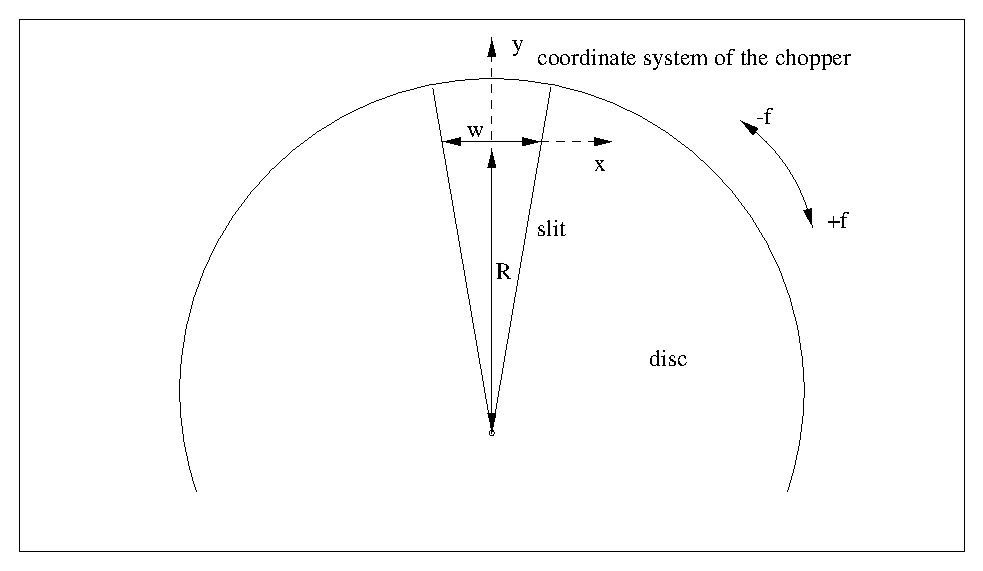
\includegraphics[width=1.0\linewidth]{figures/Chopper.eps}
\caption{disc chopper\label{f:chopper1}}
\end{figure}

Component {\bf Chopper} has $n$ openings, which are
symmetrically positioned on the disc. You can set the direction of
rotation, which allows to simulate double choppers. You can also define
the phase by setting the time at which one slit is positioned at the
top. The sides of the slits are pointing towards the center of the disc.
The thickness of the disc is neglected.  There is no parameter for the
size of the slits in the radial direction; 
use e.g. a {\bf Slit} component in front of the chopper.

Using a rectangular shaped beam with nearly the same
size as the slit, yields an almost triangular shaped
transmission curve (see figure~\ref{f:chopper2}).

\begin{figure}[ht]
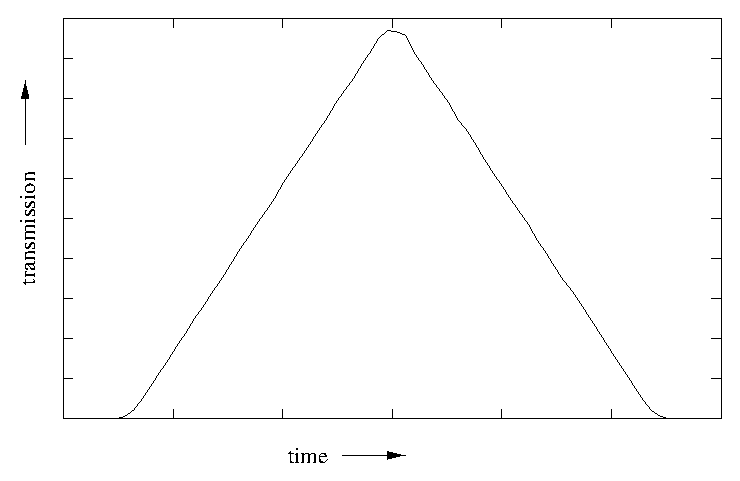
\includegraphics[width=1.0\linewidth]{figures/tracho.eps}
\caption{example transmission curve for the disc chopper\label{f:chopper2}}
\end{figure}    

When simulating the chopping of a continuous beam,
most of the neutrons could easily be lost.
To improve efficiency, one can set the flag \verb+IsFirst+, which will
allow every neutron ray to pass the {\bf Chopper}, but modify the 
time, $t$, to a time at which it is possible to pass. 
This can also be used with TOF-instruments, which often
define the starting time of the neutrons at
the position of the first chopper.
Of course, there should be only one ``first chopper'' in
any simulation.
To simulate frame overlap from a ``first chopper'', one can specify 
the number of frames to study by the parameter $n_{\rm pulse}$.
% Emacs settings: -*-mode: latex; TeX-master: "manual.tex"; -*-

\section{Detectors and monitors}

In real neutron experiments, detectors and monitors play quite
different roles. One wants the detectors to be as efficient as 
possible, counting all neutrons (and absorbing them in the process), 
while the monitors measure the intensity of the incoming beam, and must
as such be almost transparent, interacting only with (roughly) 0.1-1\%
of the neutrons passing by. In computer simulations, it is 
of course possible to detect every neutron without 
absorbing it or disturbing any of its parameters. Hence, the two components
have very similar functions in the simulations, and we do
not distinguish between them. For simplicity, they are from here on
just called monitors, since they do not absorb the neutron.

Another difference between computer simulations and real experiments is
that one may allow the monitor to be sensitive to any neutron property,
as {\em e.g.} direction, energy, and polarization, in addition to what
is found in advanced existing monitors (space and time).  One may, in
fact, let the monitor have several of these properties at the same time,
as seen for example in the energy sensitive monitor in
section~\ref{s:e_monitor}.

\subsection{Monitor: The single monitor}
The component {\bf Monitor}
consists of a rectangular opening --- like that for {\bf slit}.
The neutron is propagated to the plane of the monitor
by the kernel call PROP\_Z0.
Any neutron that passes within the opening is counted ---
the number counting variable is incremented: $N_i = N_{i-1}+1$,
the neutron
weight $p_i$ is added to the weight counting variable:
$I_i = I_{i-1} + p_i$, 
and the second moment of the weight is
updated: $M_{2,i} = M_{2,i-1} + p_i^2$. 
The input parameters for {\bf Monitor} are
the opening coordinates $x_{\rm min}, x_{\rm max}, y_{\rm min}$, 
$y_{\rm max}$, 
and the output parameters are the three count numbers, $N, I$, and $M_2$.

\subsection{Monitor\_4PI: The $4\pi$ monitor}
The component {\bf Monitor\_4PI} does not model any physical monitor
but may be thought of as a spherical monitor completely surrounding the
previous component. 
It simply detects all neutrons that have not been absorbed at the
position in the instrument in which it is placed.
If this monitor is placed in the instrument file after
another component, {\em e.g.} a sample,
it will count any neutron scattered from this component.
This may be useful during tests.

The output parameters for {\bf Monitor\_4PI} are the three count numbers, $N, I$, and $M_2$.

\subsection{PSD\_monitor: The PSD monitor}
The component {\bf PSD\_monitor} closely resembles 
{\bf Monitor}.
In the PSD monitor, though, the rectangular monitor window is divided
into $n \times m$ pixels, each of which acts like a single
monitor.

The input parameters for {\bf PSD\-monitor} are
the opening coordinates $x_{\rm min}, x_{\rm max}, y_{\rm min}$, 
$y_{\rm max}$, the array dimensions $(n,m)$, and a name of a file in
which to store $I(x,y)$.
The output parameters are three two-dimensional arrays 
of counts: $N(x,y), I(x,y), M_2(x,y)$.

\subsection{PSD\_monitor\_4PI: The $4\pi$ PSD monitor}
The component {\bf PSD\_monitor\_4PI} represents 
a PSD monitor shaped as a sphere, much like {\bf Monitor\_4PI}.
It subdivides the surface of the sphere into pixels of equal 
area (using a projection onto a cylinder with an axis
which is vertical in the local coordinate system) 
and distributes the incoming neutron counts into the respective pixels.

The $4\pi$ PSD monitor is typically placed
around another component. Used in this way, 
the $4\pi$ PSD monitor is very useful for debugging components.

The input parameters for {\bf PSD\_monitor\_4PI} are
the monitor radius, the number of pixels, $(n_x, n_y)$ -- where
$y$ is the vertical direction, and the name of the file in which
to store $I(x,y)$. 
The output parameters of the component are the three count arrays
$N(x,y), I(x,y)$, and $M_2(x,y)$. 


\subsection{PSD\_monitor\_4PI\_log: The $4\pi$ PSD monitor with log scale}

The component {\bf PSD\_monitor\_4PI\_log} is the same as PSD\_monitor\_4PI
described in the previous section, except that the output histograms
contain the base-10 logarithm of the intensities rather than the
intensities themselves. Currently, this does not work well together with
the McStas mechanism to output detector results (see section~\ref{s:DETECTOR_OUT}), so
the total intensity as output by McStas from this detector component
will be wrong. However, the component was sufficiently useful in
Laue-type diffraction instruments to be included here nevertheless. A
future version of McStas may implement a better way to get log-scale in
output files.

The input parameters for PSD\_monitor\_4PI\_log are the same as for PSD\_monitor\_4PI.


\subsection{TOF\_monitor: The time-of-flight monitor}
{\bf TOF\_monitor} is a rectangular single monitor 
which is sensitive to
the absolute time, where the neutron is hits the component.
Like in a real time-of-flight detector, the time dimension is
binned into small time intervals of length $dt$, whence this monitor
updates a one-dimensional array of counts.

The input parameters for {\bf TOF\_monitor} are the opening 
coordinates $x_{\rm min}, x_{\rm max}, y_{\rm min}$, $y_{\rm max}$, 
the number of time bins (beginning from $t=0$),  
${\it n_{\rm chan}}$, the time spacing between bins, $dt$ (in $\mu$s), 
and the name of the output file. Output parameters of the component
are the three count arrays $N(i), I(i)$, and $M_2(i)$, where $i$ is
the bin number. 

\subsection{E\_monitor: The energy sensitive monitor}
\label{s:e_monitor}
The component {\bf E\_monitor} resembles {\bf TOF\_monitor}
to a very large extent. Only this monitor is sensitive to
the neutron energy, which in binned in \textit{nchan} bins between
$E_{\rm min}$ and $E_{\rm max}$.

The input parameters for {\bf E\_monitor} are the opening
coordinates $x_{\rm min}, x_{\rm max}, y_{\rm min}$, $y_{\rm max}$,
the total energy interval given by $E_{\rm min}$ and $E_{\rm max}$ (in meV), and
\textit{nchan} and the
name of the output file. Output parameters of the component
are the three count arrays
$N(i), I(i)$, and $M_2(i)$, $i$ being the bin number. 


\subsection{L\_monitor: The wavelength sensitive monitor}
\label{s:L_monitor}
The component {\bf L\_monitor} is a rectangular monitor with an opening
in the \textit{x-y} plane which is sensitive to the neutron wavelength.
The wavelength spectrum is output in a one-dimensional histogram.
Only neutrons with
wavelength $\lambda_0 < \lambda < \lambda_1$ are detected.

The input parameters for {\bf L\_monitor} are the opening
coordinates \textit{xmin}, \textit{xmax}, \textit{ymin}, and
\textit{ymax} defining the edges of the slit in meters;
the lower and upper wavelength limit \textit{Lmin} and
\textit{Lmax} in {\AA}ngstr{\o}m; the number of histogram bins
\textit{nchan}; and \textit{filename}, a
string giving the name of the file to store the data in.


\subsection{Divergence\_monitor: The divergence sensitive monitor}

The component {\bf Divergence\_monitor} is a rectangular monitor
with an opening in the \textit{x-y} plane,
which is sensitive to the neutron divergence, {\em i.e.} the angle
between the neutron path and the monitor surface normal.
 
The divergence is divided into horisontal and vertical divergencies,
which are calculated as $\delta_h = \tan^{-1}(v_x/v_z)$ 
and $\delta_v = \tan^{-1}(v_y/v_z)$, respectively. 
Only neutrons within a divergence window of 
$\delta_h = (-\delta_{\rm h,max} ; \delta_{\rm h,max})$, 
$\delta_v = (-\delta_{\rm v,max} ; \delta_{\rm v,max})$ 
are detected. The counts are binned in an array of $n_h \times n_v$ pixels.

The input parameters for the Divergence\_monitor component are the opening coordinates
$(x_{\rm min}, x_{\rm max}, y_{\rm min}, y_{\rm max})$, 
the number of pixels $(n_h, n_v)$, 
the parameters $(\delta_{\rm h,max}, \delta_{\rm v,max})$ 
defining the divergence interval,
and a name of the file in which to store the detected intensities.

Note that a divergence sensitive monitor with a small opening may be 
thought of as a non-reversing pinhole camera.


\subsection{DivPos\_monitor: The divergence-position sensitive monitor}

The component {\bf DivPos\_monitor} is a rectangular monitor with an
opening in the \textit{x-y} plane, which is sensitive to both the
horizontal neutron divergence and the horizontal neutron position. The
neutron intensity as a function of position and divergence is output in
a two-dimensional histogram. This output may be directly compared to an
acceptance diagram, an analytical technique that is sometimes used to
calculate neutron guide performances.
 
The horizontal divergence is calculated as $\delta_h = \tan^{-1}(v_x/v_z)$ .
Only neutrons within a divergence window of 
$\delta_h = (-\delta_{\rm h,max} ; \delta_{\rm h,max})$ are detected.

The input parameters for the DivPos\_monitor component are the opening coordinates
\textit{xmin}, \textit{xmax}, \textit{ymin}, and
\textit{ymax} in meters;
the number of histogram bins \textit{npos} and \textit{ndiv} in
position and divergence; the maximum divergence \textit{maxdiv} to
detect, in degrees; and \textit{filename}, a
string giving the name of the file to store the data in.


\subsection{DivLambda\_monitor: The divergence-wavelength sensitive monitor}

The component {\bf DivLambda\_monitor} is a rectangular monitor
with an opening in the \textit{x-y} plane,
which is sensitive to both the horizontal neutron divergence and the
wavelength. The neutron intensity as a function of wavelength and
divergence is output in a two-dimensional histogram.
 
The horizontal divergence is calculated as $\delta_h = \tan^{-1}(v_x/v_z)$ .
Only neutrons within a divergence window of 
$\delta_h = (-\delta_{\rm h,max} ; \delta_{\rm h,max})$ and with
wavelength $\lambda_0 < \lambda < \lambda_1$ are detected.

The input parameters for the DivLambda\_monitor component are the opening coordinates
\textit{xmin}, \textit{xmax}, \textit{ymin}, and
\textit{ymax} in meters;
the number of histogram bins \textit{nlam} and \textit{ndiv} in
wavelength and divergence; the maximum divergence \textit{maxdiv} to
detect, in degrees; \textit{lambda\_0} and \textit{lambda\_1} to define
the wavelength window, in {\AA}ngstr{\o}m; and \textit{filename}, a
string giving the name of the file to store the data in.


\section{Monitor\_nD: A general Monitor for 0D/1D/2D records}
\label{s:monitornd}
\index{Monitors!The All-in-One monitor (Monitor\_nD)}

\component{Monitor\_nD}{System, E. Farhi}{$x_{\rm min}$, $x_{\rm max}$, $y_{\rm min}$, $y_{\rm max}$, options}{$file$, $x_{width}, y_{height}, z_{depth}$, $bins$, $min$, $max$}{}

The component {\bf Monitor\_nD} is a general Monitor that may output any
set of physical parameters regarding the passing neutrons. The
generated files are either a set of 1D signals ([Intensity] {\it vs.}
[Variable]), or a single 2D signal ([Intensity] {\it vs.} [Variable 1]
{\it vs.} [Variable 1]), and possibly a simple long list of selected
physical parameters for each neutron.

The input parameters for {\bf Monitor\_nD} are its dimensions $x_{\rm
  min}, x_{\rm max}, y_{\rm min}$, $y_{\rm max}$ (in meters) and an {\it
  options} string describing what to detect, and what to do with the
signals, in clear language. The $x_{width}, y_{height}, z_{depth}$ may also be used to enter dimensions.

Eventhough the possibilities of Monitor\_nD are numerous, its usage remains as simple as possible, specially in the \verb+options+ parameter, which 'understands' normal language.
The formatting of the {\it options}
parameter is free, as long as it contains some specific keywords, that
can be sometimes followed by values. The {\it no} or {\it not} option
modifier will revert next option. The {\it all} option can also affect a
set of monitor configuration parameters (see below).

As the usage of this component enables to monitor virtually anything, and thus the combinations of options and parameters is infinite, we shall only present the most basic configuration. The reader should refer to the on-line component help, using e.g. \verb+mcdoc Monitor_nD.comp+.

\subsection{The Monitor\_nD geometry}

The monitor shape can be selected among seven geometries:
\begin{enumerate}
\item{({\it square}) The default geometry is flat rectangular in ($xy$)
    plane with dimensions $x_{\rm min}, x_{\rm max}, y_{\rm min}$,
    $y_{\rm max}$, or $x_{width}, y_{height}$.}
\item{({\it box}) A rectangular box with dimensions $x_{width}, y_{height}, z_{depth}$.}
\item{({\it disk}) When choosing this geometry, the detector is a flat
    disk in ($xy$) plane. The radius is then
    \begin{equation}
      \mbox{radius} = \max ( \mbox{abs } [ x_{\rm min}, x_{\rm max}, y_{\rm
        min}, y_{\rm max}, x_{width}/2, y_{height}/2 ] ).
    \end{equation}
    }
\item{({\it sphere}) The detector is a sphere with the same radius as
    for the {\it disk} geometry.}
\item{({\it cylinder}) The detector is a cylinder with revolution axis
    along $y$ (vertical). The radius in ($xz$) plane is
    \begin{equation}
      \mbox{radius} =  \max ( \mbox{abs } [ x_{\rm min}, x_{\rm max}, x_{width}/2 ] ),
    \end{equation}
    and the height along $y$ is
    \begin{equation}
      \mbox{height} =  | y_{\rm max} - y_{\rm max} | {\rm or} y_{height}.
    \end{equation}
    }
\item{({\it banana}) The same as the cylinder, but without the top/bottom caps, and on a restricted angular range. The angular range is specified using a \verb+theta+ variable limit specification in the \verb+options+.}
\item{({\it previous}) The detector has the shape of the previous component. This may be a surface or a volume. In this case, the neutron is detected on previous component, and there is not neutron propagation.}
\end{enumerate}

By default, the monitor is flat, rectangular. Of course, you can choose
the orientation of the {\bf Monitor\_nD} in the instrument description
file with the usual \texttt{ROTATED} modifier.

For the {\it box}, {\it sphere} and {\it cylinder}, the outgoing neutrons are
monitored by default, but you can choose to monitor incoming neutron
with the {\it incoming} option.

At last, the {\it slit} or {\it absorb} option will ask the component to
absorb the neutrons that do not intersect the monitor. The {\it exclusive} option word removes neutrons which are similarly outside the monitor limits (that may be other than geometrical).

The {\it parallel} option keyword is of common use in the case where the {\bf Monitor\_nD} is superposed with other components. It ensures that neutrons are detected independently of other geometrical constrains. This is generally the case when you need e.g. to place more than one monitor at the same place.

\subsection{The neutron parameters that can be monitored}

There are many different variables that can be monitored at the same time
and position. Some can have more than one name (e.g. \texttt{energy} or
\texttt{omega}).


\begin{verbatim}
    kx ky kz k wavevector [Angs-1] (    usually axis are
    vx vy vz v            [m/s]         x=horz., y=vert., z=on axis)
    x y z                 [m]      Distance, Position
    kxy vxy xy radius     [m]      Radial wavevector, velocity and position
    t time                [s]      Time of Flight
    energy omega          [meV]
    lambda wavelength     [Angs]
    p intensity flux      [n/s] or [n/cm^2/s]
    ncounts               [1]
    sx sy sz              [1]      Spin
    vdiv ydiv dy          [deg]    vertical divergence (y)
    hdiv divergence xdiv  [deg]    horizontal divergence (x)
    angle                 [deg]    divergence from  direction
    theta longitude       [deg]    longitude (x/z) [for sphere and cylinder]
    phi   lattitude       [deg]    lattitude (y/z) [for sphere and cylinder]
\end{verbatim}
as well as two other special variables
\begin{verbatim}
    user user1            will monitor the [Mon_Name]_Vars.UserVariable{1|2}
    user2 user3           to be assigned in an other component (see below)
\end{verbatim}

To tell the component what you want to monitor, just add the variable
names in the {\it options} parameter. The data will be sorted into {\it
  bins} cells (default is 20), between some default {\it limits}, that
can also be set by user. The {\it auto} option will automatically
determine what limits should be used to have a good sampling of signals.

\subsection{Important options}

Each monitoring records the flux (sum of weights $p$) versus the
given variables, except if the \verb+signal=<variable>+ word is used in the \verb+options+.
The {\it cm2} option will ask to normalize the flux to the monitor section surface, and the \verb+capture+ option uses the gold foil integrated 'capture' flux weightening (up to the cadmium cut-off):\index{Monitors!Capture flux}
\begin{equation}
\Phi_c = \int_0^{0.5 eV}{\frac{d\Phi}{d\lambda} \frac{\lambda}{\lambda_{2200 m/s}} d\lambda}
\end{equation}

The \verb+auto+ option is probably the most useful one: it asks the monitor to determine automatically the best limits for each variable, in order to obtain the most significant monitored histogram. This option should preceed each variable, or be located after all variables in which case they are all affected.
On the other hand, one may manually set the limits with the \verb+limits=[min max]+ option.

The \verb+log+ and \verb+abs+ options should be positioned before each variable to specify logarithmic binning and absolute value respectively.

The {\it borders} option will monitor variables that are outside
the limits. These values are then accumulated on the 'borders' of the
signal.

\subsection{The output files}

By default, the file names will be the component name, followed by a time stamp and
automatic extensions showing what was monitored (such as
\texttt{MyMonitor.x}). You can also set the filename in {\it options}
with the {\it file} keyword followed by the file name that you want. The
extension will then be added if the name does not contain a dot (.).
Finally, the $filename$ parameter may also be used.

The output files format are standard 1D or 2D McStas detector files.
The {\it no file} option will {\it unactivate} monitor, and make it a
single 0D monitor detecting integrated flux and counts.
The {\it verbose} option will display the nature of the monitor, and the
names of the generated files.

\subsubsection{The 2D output}

When you ask the {\bf Monitor\_nD} to monitor only two variables (e.g.
{\it options} = "x y"), a single 2D file of intensity versus these two
correlated variables will be created.

\subsubsection{The 1D output}

The {\bf Monitor\_nD} can produce a set of 1D files, one for each
monitored variable, when using 1 or more than 2 variables, or when
specifying the {\it multiple} keyword option.

\subsubsection{The List output}

The {\bf Monitor\_nD} can additionally produce a {\it list} of variable
values for neutrons that pass into the monitor. This feature is additive
to the 1D or 2D output. By default only 1000 events will be recorded in
the file, but you can specify for instance "{\it list} 3000 neutrons" or
"{\it list all} neutrons". This last option might require a lot of
memory and generate huge files.

\subsection{Monitor equivalences}

In the following table \ref{t:monitor-nd-equiv}, we show how the Monitor\_nD may substitute any other \MCS monitor.

\begin{table}
  \begin{center}
    {\let\my=\\
    \begin{tabular}{|p{0.24\textwidth}|p{0.7\textwidth}|}
\hline
\MCS monitor & Monitor\_nD equivalent \\
\hline
Divergence\_monitor & {\it options}="dx bins=$ndiv$ limits=[$-\alpha/2 \alpha/2$],
                                lambda bins=$nlam$ limits=[$\lambda_0$ $\lambda_1$] file=$file$"\\
DivLambda\_monitor  & {\it options}="dx bins=$nh$   limits=[$-h_{max}/2 h_{max}/2$],
                                    dy bins=$nv$   limits=[$-v_{max}/2 v_{max}/2$]" {\it filename}=$file$\\
DivPos\_monitor     & {\it options}="dx bins=$ndiv$ limits=[$-\alpha/2 \alpha/2$],
                                     x bins=$npos$" {\it xmin}=$x_{min}$ {\it xmax}=$x_{max}$ \\
E\_monitor          & {\it options}="energy bins=$nchan$ limits=[$E_{min} E_{max}$]" \\
EPSD\_monitor       & {\it options}="energy bins=$n_E$ limits=[$E_{min} E_{max}$], x bins=$nx$"
                              {\it xmin}=$x_{min}$ {\it xmax}=$x_{max}$ \\
Hdiv\_monitor       & {\it options}="dx bins=$nh$ limits=[$-h_{max}/2 h_{max}/2$]" {\it filename}=$file$ \\
L\_monitor          & {\it options}="lambda bins=$nh$ limits=[$-\lambda_{max}/2 \lambda_{max}/2$]" {\it filename}=$file$ \\
Monitor\_4PI        & {\it options}="sphere" \\
Monitor            & {\it options}="unactivate" \\
PSDcyl\_monitor     & {\it options}="theta bins=$nr$,y bins=$ny$, cylinder"
{\it filename}=$file$ {\it yheight}=$height$ {\it xwidth}=2*radius\\
PSDlin\_monitor     & {\it options}="x bins=$nx$" {\it xmin}=$x_{min}$ {\it xmax}=$x_{max}$ {\it ymin}=$y_{min}$ {\it ymax}=$y_{max}$ {\it filename}=$file$\\
PSD\_monitor\_4PI    & {\it options}="theta y, sphere" \\
PSD\_monitor        & {\it options}="x bins=$nx$, y bins=$ny$" {\it xmin}=$x_{min}$ {\it xmax}=$x_{max}$ {\it ymin}=$y_{min}$ {\it ymax}=$y_{max}$ {\it filename}=$file$\\
TOF\_cylPSD\_monitor & {\it options}="theta bins=$n_\phi$, time bins=$nt$ limits=[$t_0, t_1$], cylinder" {\it filename}=$file$ {\it yheight}=$height$ {\it xwidth}=2*radius\\
TOFLambda\_monitor  & {\it options}="lambda bins=$n_\lambda$ limits=[$\lambda_0$ $\lambda_1$], time bins=$nt$ limits=[$t_0, t_1$]" {\it filename}=$file$\\
TOFlog\_mon         & {\it options}="log time bins=$nt$ limits=[$t_0, t_1$]" \\
TOF\_monitor        & {\it options}="time bins=$nt$ limits=[$t_0, t_1$]" \\
\hline
    \end{tabular}
    \caption{Using Monitor\_nD in place of other components. All limits specifications may be advantageously replaced by an {\it auto} word preceeding each monitored variable. Not all file and dimension specifications are indicated (e.g. filename, xmin, xmax, ymin, ymax).}
    \label{t:monitor-nd-equiv}
    }
  \end{center}
\end{table}

\subsection{Usage examples}

\begin{itemize}
\item{
\begin{verbatim}
COMPONENT MyMonitor = Monitor_nD(
    xmin = -0.1, xmax = 0.1,
    ymin = -0.1, ymax = 0.1,
    options = "energy auto limits")
\end{verbatim}
will monitor the neutron energy in a single 1D file (a kind of E\_monitor)}
\item{\texttt{options = "banana, theta limits=[10,130], bins=120, y bins=30"} \\
    is a theta/height banana detector.\index{Monitors!Banana shape}}
\item{\texttt{options = "banana, theta limits=[10,130], auto time"} \\
    is a theta/time-of-flight banana detector.}

\item{\texttt{options="x bins=30 limits=[-0.05 0.05] ; y"} \\
    will set the monitor to look at $x$ and $y$. For $y$, default bins (20)
    and limits values (monitor dimensions) are used.}

\item{\texttt{options="x y, auto, all bins=30"} \\
    will determine itself the required limits for $x$ and $y$.}

\item{\texttt{options="multiple x bins=30, y limits=[-0.05 0.05], all auto"} \\
will monitor the neutron $x$ and $y$ in two 1D files.}
\item{\texttt{options="x y z kx ky kz, all auto"} \\
will monitor each of theses variables in six 1D files.}
\item{\texttt{options="x y z kx ky kz, list all, all auto"} \\
will monitor all theses neutron variables in one long list, one row per neutron event.}
\item{\texttt{options="multiple x y z kx ky kz, and list 2000, all auto"} \\
    will monitor all theses neutron variables in one list of 2000 events
    and in six 1D files.}
\item{\texttt{options="signal=energy, x y"} \\
    is a PSD monitor recording the mean energy of the beam as a function of $x$ and $y$.\index{Monitors!Position sensitive monitor recording mean energy}}
\end{itemize}

\subsection{Monitoring user variables}
\label{s:monnd:user}
\index{Monitors!Custom monitoring (user variables, Monitor\_nD)}

There are two ways to monitor any quantity with Monitor\_nD. This may be e.g. the number of neutron bounces in a guide, or the wavevector and energy transfer at a sample. The only requirement is to define the \verb+user1+ (and optionally \verb+user2,user3+) variables of a given Monitor\_nD instance.

\subsubsection{Setting directly the user variables (simple)}

The first method uses directly the \verb+user1+ and \verb+username1+ component parameters to transfert directly the value and label, such as in the following example:
\begin{verbatim}
TRACE
(...)
COMPONENT UserMonitor = Monitor_nD(
  user1    = log(t), username1="Log(time)",
  options  ="auto user1")
\end{verbatim}
The values to assign to \verb+user2+ and \verb+user3+ must be global instrument variables, or a component output variables as in \verb+user1=MC_GETPAR(some_comp, outpar)+.
Similarly, the \verb+user2,user3+ and \verb+username2,username3+ parameters may be used to control the second and third user variable, to produce eventually 2D/3D user variable correlation data and custom event lists.

\subsubsection{Setting indirectly the user variables (only for professionals)}

It is possible to control the user variables of a given Monitor\_nD instance anywhere in the instrument description. This method requires more coding, but has the advantage that a variable may be defined to store the result of a computation locally, and then transfert it into the UserMonitor, all fitting in an EXTEND block.

This is performed in a 4 steps process:
\begin{enumerate}
\item Declare that you intend to monitor user variables in a Monitor\_nD instance (defined in TRACE):
\begin{verbatim}
DECLARE
%{ (...)
  %include "monitor_nd-lib"
  MONND_DECLARE(UserMonitor); // will monitor custom things in UserMonitor
%}
\end{verbatim}
\item Initialize the label of the user variable (optional):
\begin{verbatim}
INITIALIZE
%{
  (...)
  MONND_USER_TITLE(UserMonitor, 1, "Log(time)");
%}
\end{verbatim}
The value '1' could be '2' or '3' for the \verb+user2,user3+ variable.
\item Set the user variable value in a TRACE component EXTEND block:\index{Keyword!EXTEND}
\begin{verbatim}
TRACE
(...)
COMPONENT blah = blah_comp(...)
EXTEND
%{  // attach a value to user1 in UserMonitor, could be much more comlex here.
  MONND_USER_VALUE(UserMonitor, 1, log(t));
%}
(...)
\end{verbatim}
\item Tell the Monitor\_nD instance to record user variables:
\begin{verbatim}
TRACE
(...)
COMPONENT UserMonitor = Monitor_nD(options="auto user1")
(...)
\end{verbatim}
\end{enumerate}
Setting the user variable values may either make use of the neutron parameters (x,y,z, vx,vy,vz, t, sx,sy,sz, p), access the internal variables of the component that sets the user variables (in this example, those from the \verb+blah+ instance), access any component OUTPUT parameter \index{Keyword!OUTPUT PARAMETERS} using the \verb+MC_GETPAR+ C macro(see chapter \ref{c:kernelcalls}), or simply use a global instrument variable. Instrument parameters can not be used directly.
\index{Library!Run-time!MC\_GETPAR}

\subsubsection{Example: Number of neutron bounces in a guide}

\index{Monitors!Number of neutron bounces in a guide}
In the following example, we show how the number of bounces in a polygonal guide may be monitored. Let us have a guide made of many Guide\_gravity instances. We declare a global simulation variable \verb+nbounces+, set it to 0 for each neutron entering the guide, and sum-up all bounces from each section, accessing the \verb+Gvars+ OUTPUT variable of component Guide\_gravity. Then we ask Monitor\_nD to look at that value.
\begin{verbatim}
DECLARE
%{
  double nbounces;
%}
TRACE
(...)
COMPONENT Guide_in = Arm() AT (...)
EXTEND
%{
  nbounces = 0;
%}

COMPONENT Guide1 = Guide_gravity(...) AT (...) RELATIVE PREVIOUS
EXTEND
%{
  if (SCATTERED) nbounces += GVars.N_reflection[0];
%}
(... many guide instances, copy/paste and change names automatically ...)
COMPONENT COPY(Guide1) = COPY(Guide1) AT (...) RELATIVE PREVIOUS
EXTEND
%{
  if (SCATTERED) nbounces += GVars.N_reflection[0];
%}

// monitor nbounces
COMPONENT UserMonitor = Monitor_nD(
  user1=nbounces, username1="Number of bounces",
  options="auto user1") AT (...)
(...)
\end{verbatim}

\subsection{Monitoring neutron parameter correlations, PreMonitor\_nD}

The first imediate usage of the Monitor\_nD component is when one requires to identify cross-correlations between some neutron parameters, e.g. position and divergence ({\it aka} phase-space diagram). This latter monitor would be merely obtained with:\index{Monitors!Neutron parameter correlations, PreMonitor\_nD}
\begin{verbatim}
options="x dx, auto", bins=30
\end{verbatim}
This example records the correlation between position and divergence of neutrons at a given instrument location.

\component{PreMonitor\_nD}{System, E. Farhi}{comp}{}{}

But it is also possible to search for cross-correlation between two part of the instrument simulation. One example is the acceptance phase-diagram, which shows the neutron caracteristics at the input required to reach the end of the simulation. This \emph{spatial} correlation may be revealed using the {\bf PreMonitor\_nD} component. This latter stores the neutron parameters at a given instrument location, to be used at an other Monitor\_nD location for monitoring.

The only parameter of {\bf PreMonitor\_nD} is the name of the associated Monitor\_nD instance, which should use the \verb+premonitor+ option, as in the following example:
\begin{verbatim}
COMPONENT CorrelationLocation = PreMonitor_nD(comp = CorrelationMonitor)
AT (...)

  (... e.g. a guide system )

COMPONENT CorrelationMonitor  = Monitor_nD(
   options="x dx, auto, all bins=30, premonitor")
AT (...)
\end{verbatim}
which performs the same monitoring as the previous example, but with a spatial correlation constrain. Indeed, it records the position {\it vs} the divergence of neutrons at the correlation location, but only if they reach the monitoring position. All usual Monitor\_nD variables may be used, except the user variables. These latter may be defined as described in section \ref{s:monnd:user} in an EXTEND block.



\subsection{Res\_monitor: The resolution monitor}
\label{s:res_monitor}
The component \textbf{Res\_monitor} is used together with the
\textbf{Res\_sample} component (described in section~\ref{s:res_sample})
and the \verb+mcresplot+ front-end (described in
section~\ref{s:mcresplot}). It works like a normal single detector, but
also records all scattering events in the resolution sample and writes
them to a file that can later be read by \verb+mcresplot+.

The instrument definition should contain an instance of the
\textbf{Res\_sample} component, the name of which should be passed as an
input parameter to \textbf{Res\_monitor}. For example
\begin{verbatim}
    COMPONENT mysample = Res_sample( ... )
    ...
    COMPONENT det = Res_monitor(res_sample_comp = mysample, ...)
    ...
\end{verbatim}

The output file is in ASCII format, one line per scattering event, with
the following columns:
\begin{itemize}
\item ${\bf k}_{\rm i}$, the three components of the initial wave vector.
\item ${\bf k}_{\rm f}$, the three components of the final wave vector.
\item ${\bf r}$, the three components of the position of the scattering
  event in the sample.
\item $p_{\rm i}$, the neutron weight just after the scattering event.
\item $p_{\rm f}$, the relative neutron weight adjustment from sample to
  detector (so the total weight in the detector is $p_{\rm i}p_{\rm f}$).
\end{itemize}
From ${\bf k}_{\rm i}$ and ${\bf k}_{\rm f}$, we may compute ${\bf Q} =
{\bf k}_{\rm i} - {\bf k}_{\rm f}$ and $\omega = (\mbox{2.072
  meV$\cdot$\AA$^2$})({\bf k}_{\rm i}^2 - {\bf k}_{\rm f}^2)$.

The vectors are given in the local coordinate system of the resolution
sample component. The wave vectors are in units of $\mbox{\AA}^{-1}$, the
scattering position in units of meters.

The input parameters for {\bf Res\_monitor} are the opening coordinates
$x_{\rm min}, x_{\rm max}, y_{\rm min}$, $y_{\rm max}$ as for the single
monitor component, the name of the file to write in \textit{filename},
and \textit{res\_sample\_comp} which should be set to the name of the
resolution sample component used in the instrument.  The output
parameters are the three count numbers, \textit{Nsum}, \textit{psum},
and \textit{p2sum}, and the handle \textit{file} of the output file.

\subsection{Adapt\_check: The simple adaptive importance sampling monitor}
\label{s:adapt_check}

The component {\bf Adapt\_check} is used together with the Source\_adapt
component --- see section~\ref{s:source_adapt} for details. When placed
somewhere in an instrument using Source\_adapt, the source will optimize
for neutrons that reach that point without being absorbed (regardless of
neutron position, direction, wavelength, \textit{etc}).

The Adapt\_check component takes a single input parameter
\textit{source\_comp}. This should be set to the name given to the
Source\_adapt component in the instrument, for example
\begin{verbatim}
  ...
  COMPONENT mysource = Source_adapt( ... )
  ...
  COMPONENT mycheck = Adapt_check(source_comp = mysource)
  ...
\end{verbatim}

% Emacs settings: -*-mode: latex; TeX-master: "manual.tex"; -*-

\section{Monitor\_Optimizer: Optimization locations for the\\
  Source\_Optimizer}
\label{monitor-optimizer}
\index{Sources!Optimization location|see{Sources/Optimizer}}\index{Optimization}
\component{Source\_Optimizer}{E. Farhi, ILL}{optim\_comp}{$x_{min}$, $x_{max}$, $y_{min}$,$y_{max}$}{partially validated}

The {\bf Monitor\_Optimizer} component works with the {\bf
  Source\_Optimizer} component. See section~\ref{source-optimizer}
for usage.

The input parameters for {\bf Monitor\_Optimizer} are the rectangular
shaped opening coordinates $x_{min}$, $x_{max}$, $y_{min}$,
$y_{max}$, and the name of the associated instance of
{\bf Source\_Optimizer} used in the instrument description file (one word,
without quotes).

As many Monitor\_Optimizer instances as required may be used in an instrument, 
for possibly more than one optimization location. 
Multiple instances may all have an effect on the total intensity.


% Emacs settings: -*-mode: latex; TeX-master: "manual.tex"; -*-

\chapter{Bragg scattering single crystals, monochromators}

In this class of components, we are concerned with elastic Bragg
scattering from single crystals. The Mosaic\_anisotropic component
models a thin mosaic crystal with a single scattering vector
perpendicular to the surface. It is a replacement for the Monochromator
component from previous releases; it uses a better algorithm that works
in some cases where the old component would give wrong results. The
Mosaic\_simple component is similar, but has an isotropic mosaic and
allows a scattering vector that is not perpendicular to the surface. The
Single\_crystal component is a general single crystal sample that allows
the input of an arbitrary unit cell and a list of structure factors, and
also allows anisotropic mosaic and $\Delta d/d$ lattice space variation.

% Emacs settings: -*-mode: latex; TeX-master: "manual.tex"; -*-

\subsection{Mosaic\_simple: An infinitely thin mosaic crystal with a single scattering
  vector}
\label{s:mosaic-simple}

The component {\bf Mosaic\_simple} simulates an infinitely thin single
crystal with a single scattering vector and a mosaic spread. A typical
use for this component is to simulate a monochromator or an analyzer.

The physical model used in the component is a rectangular piece of
material composed of a large number of small micro-crystals.
The orientation of the
micro-crystals deviates from the nominal crystal orientation so that the
probability of a given micro-crystal orientation is proportional to a
Gaussian in the angle between the given and the nominal orientation. The
width of the Gaussian is given by the mosaic spread of the crystal. The
mosaic spread is assumed to be large compared to the Bragg width of the
scattering vector.

As a further simplification, the crystal is assumed to be infinitely
thin. This means that multiple scattering effects are not simulated. It
also means that the total reflectivity can be used as a parameter for
the model rather than the atomic scattering cross section. The variance
of the lattice spacing ($\Delta d/d$) is assumed to be zero, so this
component is not suitable for simulating backscattering instruments (use
the component Single\_crystal in section~\ref{s:Single_crystal} for that).

When a neutron trajectory intersects the crystal, the first step in the
computation is to determine the probability of scattering. This
probability is then used in a Monte Carlo choice deciding whether to
scatter or transmit the neutron. The scattering probability is the sum
of the probabilities of first-order scattering, second-order, \ldots, up
to the highest order that permits Bragg scattering at the given neutron
wave length. However, in most cases at most one order will have a
significant scattering probability, and the computation thus considers
only the order that best matches the neutron wavelength. Bragg's law is
%
$$ n{\bf Q}_0 = 2{\bf k}_i\sin\theta $$
%
Thus, the scattering order is obtained simply as the integer multiple
$n$ of the nominal scattering vector ${\bf Q}_0$ which is closest to the
projection of $2{\bf k}_i$ onto ${\bf Q}_0$ (see
figure~\ref{f:mosaic_order}).
%  k=2PI/lambda
%  q=2k sin(theta)
%  
%  2 PI n/k = d q/2k
%  q = n 4 PI/d
%  
%  n 2PI/k = n 4 PI/q \sin\theta
%  1/k = 2/q\sin\theta
%  n q = 2k\sin\theta
\begin{figure}
  \begin{center}
    \psfrag{theta}[l][l]{$\theta$}
    \psfrag{ki}[r][r]{$2{\bf k}_{\rm i}$}
    \psfrag{Q0}[l][l]{${\bf Q}_0$}
    \psfrag{2Q0}[l][l]{$2{\bf Q}_0$}
    \psfrag{3Q0}[l][l]{$3{\bf Q}_0$}
    \psfrag{4Q0}[l][l]{$4{\bf Q}_0$}
    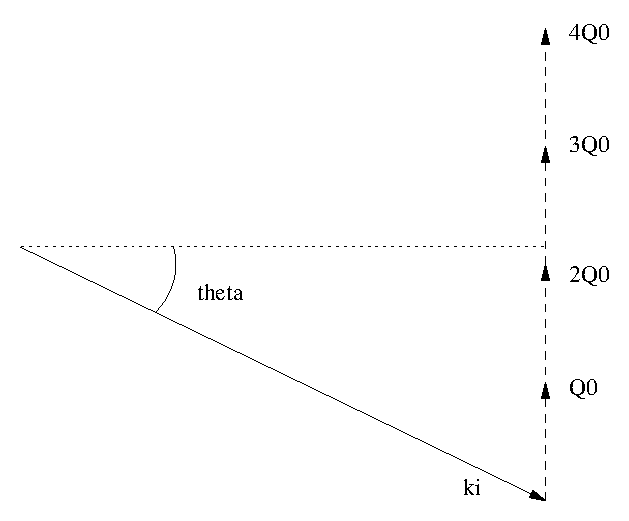
\includegraphics[width=0.5\textwidth]{figures/mosaic_order.eps}
  \end{center}
\caption{Selection of the Bragg order (``2'' in this case).}
\label{f:mosaic_order}
\end{figure}
%
Once $n$ has been determined, the Bragg angle $\theta$ can be
computed. The angle $d$ that the nominal scattering vector ${\bf Q}_0$
makes with the closest scattering vector ${\bf q}$ that admits Bragg
scattering is then used to compute the probability of reflection from
the mosaic
$$ p_{\rm reflect} = R_0 e^{-d^2/2\sigma^2}, $$
where $R_0$ is the reflectivity at the Bragg angle (see
figure~\ref{f:mosaic_angle}). The probability $p_{\rm reflect}$ is used
in a Monte Carlo choice to decide whether the neutron is transmitted or
reflected.
%
\begin{figure}
  \begin{center}
    \psfrag{th}[r][r]{$\theta$}
    \psfrag{ki}[r][r]{$2{\bf k}_{\rm i}$}
    \psfrag{kf}[l][l]{$2{\bf k}_{\rm f}$}
    \psfrag{Q0}[l][l]{${\bf Q}_0$}
    \psfrag{d}[c][c]{$d$}
    \psfrag{q}[l][l]{$\bf q$}
    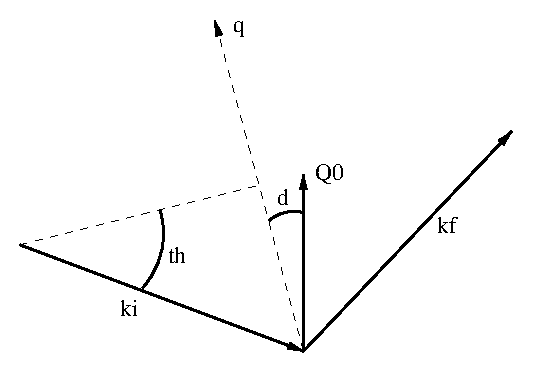
\includegraphics[width=0.5\textwidth]{figures/mosaic_angle.eps}
  \end{center}
\caption{Computing the deviation $d$ from the nominal scattering direction.}
\label{f:mosaic_angle}
\end{figure}

In the case of reflection, the neutron will be scattered into the
Debye-Scherrer cone, with the probability of each point on the cone
being determined by the mosaic. The Debye-Scherrer cone can be described
by the equation
\begin{equation}
  \label{eq:mosaic_cone}
  {\bf k}_{\rm f} = {\bf k}_{\rm i}\cos2\theta +
      \sin2\theta({\bf c}\cos\varphi + {\bf b}\sin\varphi),
      \qquad\varphi\in[-\pi;\pi],
\end{equation}
where ${\bf b}$ is a vector perpendicular to ${\bf k}_{\rm i}$ and ${\bf
Q}_0$, ${\bf c}$ is perpendicular to ${\bf k}_{\rm i}$ and ${\bf b}$,
and both ${\bf b}$ and ${\bf c}$ have the same length as ${\bf k}_{\rm
  i}$ (see figure~\ref{f:mosaic_cone}). When choosing $\varphi$ (and
thereby ${\bf k}_{\rm f}$), only a small part of the full $[-\pi; \pi]$
range will have appreciable scattering probability in non-backscattering
configurations. The best statistics is thus obtained by sampling
$\varphi$ only from a suitably narrow range.

The (small) deviation angle $\sigma$ of ${\bf q}$ from the nominal
scattering vector $n{\bf Q}_0$ corresponds to a $\Delta q$ of
$$ \Delta q \approx \sigma 2k\sin\theta. $$
The angle $\varphi$ corresponds to a $\Delta k_{\rm f}$ (and hence
$\Delta q$) of
$$ \Delta q \approx \varphi k \sin(2\theta) $$
(see figure~\ref{f:mosaic_cone}).
Hence we may sample $\varphi$ from a Gaussian with standard deviation
$$ \sigma\frac{2k\sin\theta}{k\sin(2\theta)} =
\sigma\frac{2k\sin\theta}{2k\sin\theta\cos\theta} =
\frac{\sigma}{\cos\theta} $$
to get good statistics.
%
\begin{figure}
  \begin{center}
    \psfrag{th}[r][r]{$2\theta$}
    \psfrag{ki}[c][c]{$2{\bf k}_{\rm i}$}
    \psfrag{kf}[r][r]{$2{\bf k}_{\rm f}$}
    \psfrag{nQ0}[l][l]{$n{\bf Q}_0$}
    \psfrag{q}[l][l]{$\bf q$}
    \psfrag{2ksin2t}[l][l]{$2 k \sin(2 \theta)$}
    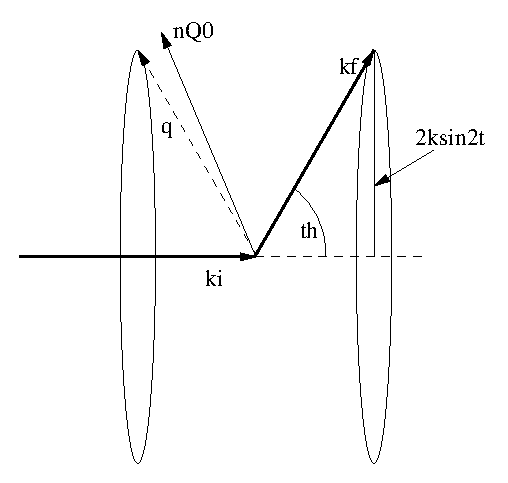
\includegraphics[width=0.5\textwidth]{figures/mosaic_cone.eps}
  \end{center}
\caption{Scattering into the part of the Debye-Scherrer cone covered by
    the mosaic.}
\label{f:mosaic_cone}
\end{figure}

What remains is to get the neutron weight right. The distribution from
which the scattering event is sampled is a Gaussian in $\varphi$ of
width $\frac{\sigma}{\cos\theta}$,
$$ f_{\rm MC}(\varphi) = \frac{1}{\sqrt{2\pi}(\sigma/\cos\theta)}
            e^{-\varphi^2/2(\sigma/\cos\theta)^2}
$$
In the physical model, the probability of the scattering event is
proportional to a Gaussian in the angle between the nominal scattering
vector ${\bf Q}_0$ and the actual scattering vector ${\bf q}$. The
normalization condition is that the integral over all $\varphi$ should
be 1. Thus the probability of the scattering event in the physical model
is
\begin{equation}
  \label{eq:mosaic_integral}
  \Pi(\varphi) = e^{\frac{-d(\varphi)^2}{2\sigma^2}} /
   \int_{-\pi}^{\pi} e^{\frac{-d(\varphi)^2}{2\sigma^2}} d\varphi
\end{equation}
where $d(\varphi)$ denotes the angle between the nominal scattering
vector and the actual scattering vector corresponding to $\varphi$.
According to equation~(\ref{probrule}), the weight adjustment $\pi_j$ is
then given by
$$ \pi_j = \Pi(\varphi) / f_{\rm MC}(\varphi). $$
In the implementation, the integral in~(\ref{eq:mosaic_integral}) is computed
using a 15-order Gaussian quadrature formula, with the integral
restricted to an interval of width $5\sigma/\cos\theta$ for the same
reasons discussed above on the sampling of $\varphi$.

The input parameters for Mosaic\_simple are \textit{zmin},
\textit{zmax}, \textit{ymin}, and \textit{ymax} to define the surface of
the crystal in the Y-Z plane; \textit{mosaic} to give the FWHM of the
mosaic spread; \textit{R0} to give the reflectivity at the Bragg angle,
and \textit{Qx}, \textit{Qy}, and \textit{Qz} to give the scattering
vector.



\subsection{Mosaic\_anisotropic: The crystal with anisotropic mosaic}

The component {\bf Mosaic\_anisotropic} is a modified version of the
Mosaic\_simple component, intended to replace the Monocromator component
from previous releases. It restricts the scattering vector to be
perpendicular to the crystal surface, but extends the Mosaic\_simple
component by allowing different mosaics in the horizontal and vertical
direction.

The code is largely similar to that for Mosaic\_simple, and the
documentation for the latter should be consulted for details. The
differences are mainly due to two reasons:
\begin{itemize}
\item Some simplifications have been done since two of the components of
  the scattering vector are known to be zero.
\item The computation of the Gaussian for the mosaic is done done using
  different mosaics for the two axes.
\end{itemize}

The input parameters for the component Mosaic\_anisotropic are
\textit{zmin}, \textit{zmax}, \textit{ymin}, and \textit{ymax} to define
the size of the crystal (in meters); \textit{mosaich} and \textit{mosaicv} to define
the mosaic (in minutes of arc); \textit{r0} to define the reflectivity
(no unit); and \textit{Q} to set the length of the scattering vector (in
$\mbox{\AA}^{-1}$).

\section{Single\_crystal: The single crystal component}
\label{s:Single_crystal}
\index{Samples!Single crystal diffraction}
\index{Diffraction}
\index{Incoherent elastic scattering}
\index{Multiple scattering}

\component{Single\_crystal}{Kristian Nielsen}{$x_{width}, y_{height}, z_{thick}$,$\vec a, \vec b, \vec c, \Delta d/d$, mosaic, reflections}{$\sigma_{abs}, \sigma_{inc}$, ...}{Partially validated, centered. Further validation undergoing. Known BUGS: The component is known not to work as a Bragg monochromator, likely the problem relates to the internal definition of the reciprocal space. Possibly related to this, the model of anistropic mosaic is broken - always use a non-zero isotropic mosaic. Also, always use a non-zero value of the $\Delta d/d$ parameter.}

The {\bf Single\_crystal} component models a thick, flat single crystal
with multiple scattering and absorption with elastic coherent scattering.
An elastic incoherent background may also be simulated.
It may be used to describe samples for diffraction,
but also for accurate monochromator descriptions.
The component is currently under further review. The current documentation is outdated, especially with respect to the model of crystal mosaicity.

The input parameters for the component are \textit{xwidth},
\textit{yheight}, and \textit{zthick} to define the dimensions of the
crystal in meters (area is centered); \textit{delta\_d\_d} to give the
value of $\Delta d/d$ (no unit);
$(\textit{ax}, \textit{ay}, \textit{az})$, $(\textit{bx}, \textit{by},
\textit{bz})$, and $(\textit{cx}, \textit{cy}, \textit{cz})$ to define
the axes of the direct lattice of the crystal (the sides of the unit
cell) in units of {\AA}ngstr{\o}m; and \textit{reflections}, a string
giving the name of the file with the list of structure factors to
consider.
The mosaic is specified \emph{either} isotropically as
\textit{mosaic}, \emph{or} anisotropically as \textit{mosaic\_h}
(rotation around the $Y$ axis), \textit{mosaic\_v} (rotation around the
$Z$ axis), and \textit{mosaic\_n} (rotation around the $X$ axis); in all
cases in units of full-width-half-maximum minutes of arc.

Optionally, the absorption cross-section at 2200 m/s and the incoherent
cross-section may be given as \textit{absorption} and
\textit{incoherent} (in barns), with default of zero; and
\textit{p\_transmit} may be assigned a fixed Monte Carlo probability for
transmission through the crystal without any interaction.

The user must specify a list of reciprocal lattice vectors
$\boldsymbol{\tau}$ to consider along with their structure factors
$|F_{\boldsymbol{\tau}}|^2$. The user must also specify the coordinates
(in direct space) of the unit cell axes $\boldsymbol{a}$,
$\boldsymbol{b}$, and $\boldsymbol{c}$, from which the reciprocal lattice
will be computed. See section \ref{s:Single_crystal_implement} for file format specifications.

In addition to coherent scattering, {\bf Single\_crystal} also
handles incoherent scattering and absorption. The incoherent scattering
cross-section is supplied by the user as a constant
$\sigma_{\rm inc}$. The absorption cross-section is supplied by the user at
2200~m/s, so the actual cross-section for a neutron of velocity $v$ is
$\sigma_{\rm abs} = \sigma_{2200} \frac{\rm 2200~m/s}{v}$.

\subsection{The physical model}

The textbook expression for the scattering cross-section of a crystal
is~\cite[ch.3]{squires}:
\begin{equation}
\label{eq:sigma_coh_el}
\left(\frac{d\sigma}{d\Omega}\right)_{\rm coh.el.} =
        N\frac{(2\pi)^3}{V_0}\sum_{\boldsymbol{\tau}}
        \delta(\boldsymbol{\tau} - \boldsymbol{\kappa})|F_{\boldsymbol{\tau}}|^2
\end{equation}
Here $|F_{\boldsymbol{\tau}}|^2$ is the structure factor
(defined in section~\ref{powder}), $N$ is the
number of unit cells, $V_0$ is the volume of an
individual unit cell, and $\boldsymbol{\kappa} (= {\bf k}_i - {\bf k}_f)$
is the scattering vector. $\delta(\boldsymbol{x})$ is a 3-dimensional delta
function in reciprocal space,
so for given incoming wave vector ${\bf k}_i$ and lattice vector
${\boldsymbol{\tau}}$, only a single final wave vector ${\bf k}_f$ is allowed.
In general, this wavevector will not fulfill the conditions for elastic
scattering $(k_f = k_i)$.
In a real crystal, however, reflections are not perfectly sharp. Because
of imperfection and finite-size effects, there will be a small region
around $\boldsymbol{\tau}$ in reciprocal space of possible scattering vectors.

{\bf Single\_crystal} simulates a crystal with a mosaic spread
$\eta$ and a lattice plane spacing uncertainty $\Delta d/d$. In such
crystals the reflections will not be completely sharp;
there will be a small region around each reciprocal lattice point of the
crystal that contains valid scattering vectors.

We model the mosaicity and $\Delta d/d$ of the crystal with
3-dimensional Gaussian functions in reciprocal space (see
figure~\ref{fig:crystal-reciprocal-space}). Two of the axes of the
Gaussian are perpendicular to the reciprocal lattice vector $\boldsymbol{\tau}$ and model
the mosaicity. The third one is parallel to $\boldsymbol{\tau}$ and models
$\Delta d/d$. We assume that the
mosaicity is small so that the possible directions of the scattering
vector may be approximated with a Gaussian in rectangular
coordinates.
\begin{figure}[t]
  \begin{center}
    \psfrag{ki}[r][r]{$\boldsymbol{k}_{\rm i}$}
    \psfrag{kf}[l][l]{$\boldsymbol{k}_{\rm f}$}
    \psfrag{tau}[r][r]{$\boldsymbol{\tau}$}
    \psfrag{mosaic}[l][l]{$\eta$}
    \psfrag{del-d-d}[l][l]{$\Delta d/d$}
    \psfrag{Ewald}[l][l]{Ewald}
    \psfrag{Sphere}[l][l]{Sphere}
    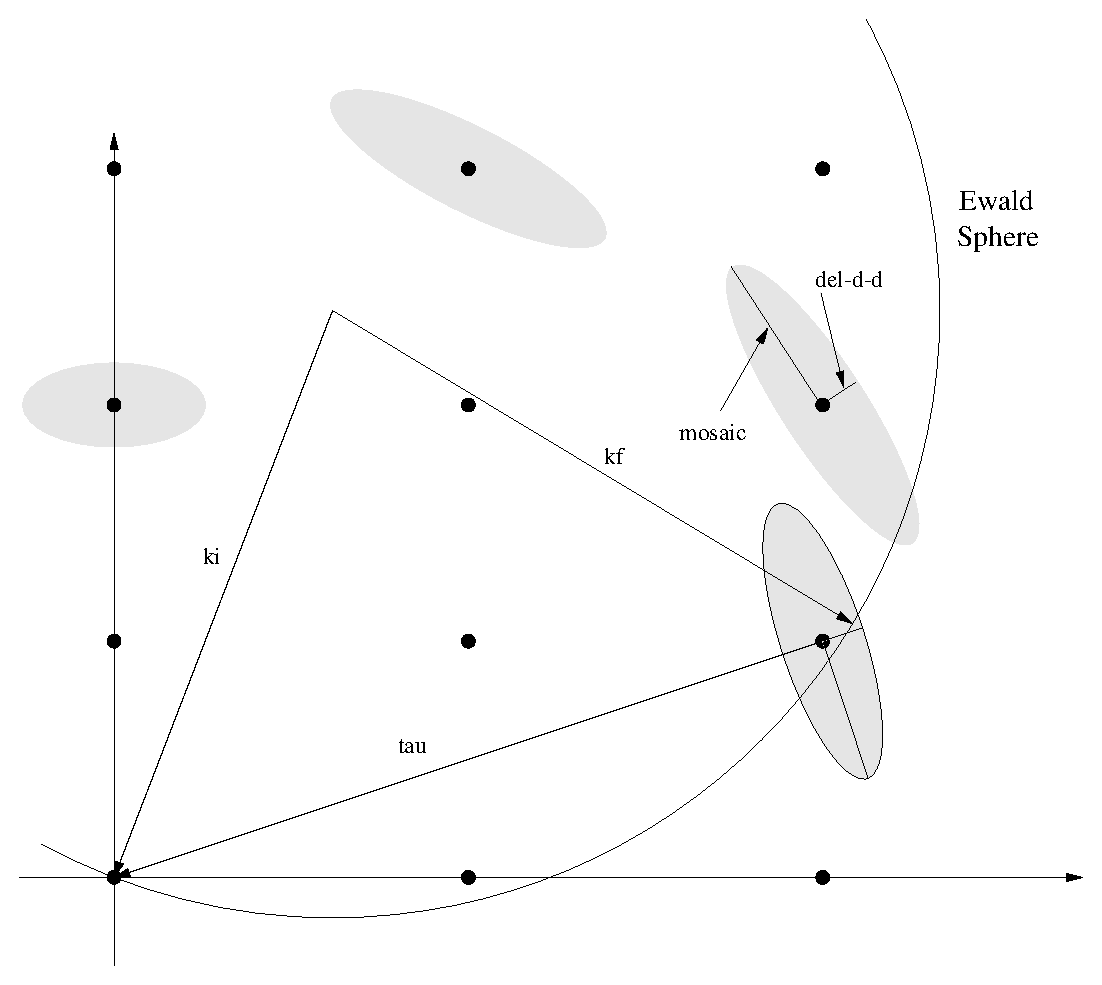
\includegraphics[width=0.7\textwidth]{figures/recip_space3.eps}
  \end{center}
\caption{Ewald sphere construction for a single neutron showing the
    Gaussian broadening of reciprocal lattice points in their local
    coordinate system.}
\label{fig:crystal-reciprocal-space}
\end{figure}

If the mosaic is isotropic (the same in all directions), the two
Gaussian axes perpendicular to $\boldsymbol{\tau}$ are simply arbitrary
normal vectors of equal length given by the mosaic. But if the mosaic
is anisotropic, the two perpendicular axes will in general be different
for each scattering vector. In the absence of anything better,
{\bf Single\_crystal} uses a model which is at least mathematically
plausible and which works as expected in the two common cases:
(1)~isotropic mosaic, and (2)~two mosaic directions (``horizontal and
vertical mosaic'') perpendicular to a scattering vector.

The basis for the model is a three-dimensional Gaussian distribution in
Euler angles giving the orientation probability distribution for the
micro-crystals; that is, the misorientation is given by small rotations
around the $X$, $Y$, and $Z$ axes, with the rotation angles having (in
general different) Gaussian probability distributions. For given
scattering vector $\boldsymbol{\tau}$, a rotation of the micro-crystals
around an axis parallel to $\boldsymbol{\tau}$ has no effect on the
direction of the scattering vector. Suppose we form the intersection
between the three-dimensional Gaussian in Euler angles and a plane
through the origin perpendicular to $\boldsymbol{\tau}$. This gives a
two-dimensional Gaussian, say with axes defined by unit vectors
$\boldsymbol{g}_1$ and $\boldsymbol{g}_2$ and mosaic widths $\eta_1$ and
$\eta_2$.

We now let the mosaic for $\boldsymbol{\tau}$ be defined by rotations
around $\boldsymbol{g}_1$ and $\boldsymbol{g}_2$ with angles having
Gaussian distributions of widths $\eta_1$ and $\eta_2$. Since
$\boldsymbol{g}_1$, $\boldsymbol{g}_2$, and $\boldsymbol{\tau}$ are
perpendicular, a small rotation of $\boldsymbol{\tau}$ around
$\boldsymbol{g}_1$ will change $\boldsymbol{\tau}$ in the direction of
$\boldsymbol{g}_2$. The two axes of the Gaussian mosaic in reciprocal
space that are perpendicular to $\boldsymbol{\tau}$ will thus be given
by $\tau\eta_2\boldsymbol{g}_1$ and $\tau\eta_1\boldsymbol{g}_2$.

We now derive a quantitative expression for the scattering cross-section
of the crystal in the model. For this, we introduce a \emph{local
  coordinate system} for each reciprocal lattice point
$\boldsymbol{\tau}$ and use $\boldsymbol{x}$ for vectors written in local
coordinates. The origin is $\boldsymbol{\tau}$, the first axis
is parallel to $\boldsymbol{\tau}$ and the other two axes are
perpendicular to $\boldsymbol{\tau}$. In the local coordinate system,
the 3-dimensional Gaussian is given by
\begin{equation}
  \label{eq:crystal-gauss-1}
  G(x_1,x_2,x_3) = \frac{1}{(\sqrt{2\pi})^3}\frac{1}{\sigma_1\sigma_2\sigma_3}
  e^{-\frac{1}{2}(\frac{x_1^2}{\sigma_1^2} +
  \frac{x_2^2}{\sigma_2^2} + \frac{x_3^2}{\sigma_3^2})}
\end{equation}
The axes of the Gaussian are $\sigma_1 = \tau\Delta d/d$ and $\sigma_2 =
\sigma_3 = \eta\tau$. Here we used the assumption that $\eta$ is small,
so that $\tan\eta \approx \eta$ (with $\eta$ given in radians).  By
introducing the diagonal matrix
$$
D = \left(
  \begin{array}[c]{ccc}
    \frac{1}{2}\sigma_1^2 & 0 & 0 \\
    0 & \frac{1}{2}\sigma_2^2 & 0 \\
    0 & 0 & \frac{1}{2}\sigma_3^2
  \end{array}\right)
$$
equation~(\ref{eq:crystal-gauss-1}) can be written as
\begin{equation}
  G(\boldsymbol{x}) =
  \frac{1}{(\sqrt{2\pi})^3}\frac{1}{\sigma_1\sigma_2\sigma_3}
  e^{-\boldsymbol{x}^{\rm T} D \boldsymbol{x}}
\end{equation}
again with $\boldsymbol{x}=(x_1,x_2,x_3)$ written in local coordinates.

To get an expression in the coordinates of the reciprocal lattice of the
crystal, we introduce a matrix $U$ such that if $\boldsymbol{y} =
(y_1,y_2,y_3)$ are the global coordinates of a point in the crystal
reciprocal lattice, then $U(\boldsymbol{y} + \boldsymbol{\tau})$ are the
coordinates in the local coordinate system for $\boldsymbol{\tau}$. The
matrix $U$ is given by
$$ U^{\rm T} = (\hat{u}_1, \hat{u}_2, \hat{u}_3), $$
where $\hat{u}_1$, $\hat{u}_2$, and $\hat{u}_3$ are the axes of the
local coordinate system, written in the global coordinates of the
reciprocal lattice. Thus
$\hat{u}_1 = \boldsymbol{\tau}/\tau$,  and $\hat{u}_2$ and $\hat{u}_3$ are
unit vectors perpendicular to $\hat{u}_1$ and to each other.
The matrix $U$ is unitarian, that is
$U^{-1} = U^{\rm T}$. The translation between global and local
coordinates is
$$ \boldsymbol{x} = U(\boldsymbol{y} + \boldsymbol{\tau}) \qquad
   \boldsymbol{y} = U^{\rm T} \boldsymbol{x} - \boldsymbol{\tau} $$

The expression for the 3-dimensional Gaussian in global coordinates is
\begin{equation}
  G(\boldsymbol{y}) =
  \frac{1}{(\sqrt{2\pi})^3}\frac{1}{\sigma_1\sigma_2\sigma_3}
  e^{-(U(\boldsymbol{y}+\boldsymbol{\tau}))^{\rm T} D (U(\boldsymbol{y}+\boldsymbol{\tau}))}
\end{equation}
The elastic coherent cross-section is then given by
\begin{equation}
  \label{eq:crystal-cross-section}
  \left(\frac{d\sigma}{d\Omega}\right)_{\rm coh.el.} =
        N\frac{(2\pi)^3}{V_0}\sum_{\boldsymbol{\tau}}
        G(\boldsymbol{\tau} - \boldsymbol{\kappa})
         |F_{\boldsymbol{\tau}}|^2
\end{equation}

\subsection{The algorithm}

The overview of the algorithm used in the Single\_crystal component is
as follows:
\begin{enumerate}
\item\label{enum:crystal-1} Check if the neutron intersects the
  crystal. If not, no action is taken.
\item\label{enum:crystal-2} Search through a list of reciprocal lattice
  points of interest, selecting those that are close enough to the Ewald
  sphere to have a non-vanishing scattering probability. From these,
  compute the total coherent cross-section $\sigma_{\rm coh}$ (see
  below), the absorption cross-section $\sigma_{\rm abs} = \sigma_{\rm
  2200} \frac{{\rm 2200~m/s}}{v}$, and the total cross-section
  $\sigma_{\rm tot} = \sigma_{\rm coh}+\sigma_{\rm inc}+\sigma_{\rm abs}$.
\item\label{enum:crystal-3} The transmission probability is
  $\exp(- \frac{\sigma_{\rm tot}}{V_0}\ell)$ where $\ell$ is the length of
  the flight path through the crystal. A Monte Carlo choice is
  performed to determine
  whether the neutron is transmitted. Optionally, the user may
  set a fixed Monte Carlo probability for the first scattering event,
  for example to boost the statistics for a weak reflection.
\item\label{enum:crystal-4} For non-transmission, the position at which
  the neutron will interact is selected from an exponential
  distribution. A Monte Carlo choice is made of whether to scatter
  coherently or incoherently. Absorption is treated by weight adjustment
  (see below).
\item\label{enum:crystal-5} For incoherent scattering, the outgoing wave
  vector $\boldsymbol{k}_{\rm f}$ is selected with a random direction.
\item\label{enum:crystal-6} For coherent scattering, a reciprocal
  lattice vector is selected by a Monte Carlo choice, and
  $\boldsymbol{k}_{\rm f}$ is found (see below).
\item\label{enum:crystal-7} Adjust the neutron weight as dictated by the
  Monte Carlo choices made.
\item\label{enum:crystal-8} Repeat from~(\ref{enum:crystal-2}) until the
  neutron is transmitted (to simulate multiple scattering).
\end{enumerate}

For point~\ref{enum:crystal-2}, the distance
\textit{dist} between a reciprocal lattice point and the Ewald sphere is
considered small enough to allow scattering if it is less than five
times the maximum axis of the Gaussian, $\textit{dist} \leq
5\max(\sigma_1,\sigma_2,\sigma_3)$.

\subsection{Choosing the outgoing wave vector}

The final wave vector $\boldsymbol{k}_{\rm f}$ must lie on the
intersection between the Ewald sphere and the Gaussian ellipsoid. Since
$\eta$ and $\Delta d/d$ are assumed small, the intersection can be
approximated with a plane tangential to the sphere, see
figure~\ref{fig:crystal-scattering-tri}. The tangential point is taken
to lie on the line between the center of the Ewald sphere
$-\boldsymbol{k}_{\rm i}$ and the reciprocal lattice point
$\boldsymbol{\tau}$. Since the radius of the Ewald sphere is $k_{\rm
  i}$, this point is
$$ \boldsymbol{o}=(k_{\rm i}/\rho - 1)\boldsymbol{\rho} - \boldsymbol{\tau} $$
where $\boldsymbol{\rho} = \boldsymbol{k}_{\rm i} - \boldsymbol{\tau}$.
\begin{figure}[t]
  \begin{center}
    \psfrag{ki}[r][r]{$\boldsymbol{k}_{\rm i}$}
    \psfrag{kf}[l][l]{$\boldsymbol{k}_{\rm f}$}
    \psfrag{rho}[r][r]{$\boldsymbol{\rho}$}
    \psfrag{tau}[r][r]{$\boldsymbol{\tau}$}
    \psfrag{x}[l][l]{$\boldsymbol{x}$}
    \psfrag{Ewald}[r][r]{Ewald}
    \psfrag{Sphere}[r][r]{Sphere}
    \psfrag{Tangential}[l][l]{Tangential}
    \psfrag{plane}[l][l]{plane}
    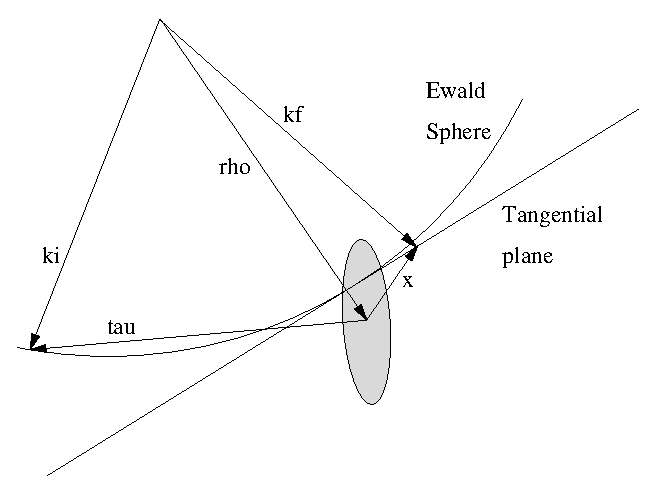
\includegraphics[width=0.7\textwidth]{figures/recip-detail.eps}
  \end{center}
\caption{The scattering triangle in the single crystal.}
\label{fig:crystal-scattering-tri}
\end{figure}

The equation for the plane is
\begin{equation}
  \label{eq:crystal-tangent-plane}
    \boldsymbol{P}(\boldsymbol{t}) = \boldsymbol{o} + B \boldsymbol{t}, \qquad
    \boldsymbol{t} \in \mathbb{R}^2
\end{equation}
Here $B = (\boldsymbol{b}_1, \boldsymbol{b}_2)$ is a $3\times 2$ matrix
with the two generators for the plane $\boldsymbol{b}_1$ and
$\boldsymbol{b}_2$. These are (arbitrary) unit vectors in the plane,
being perpendicular to
each other and to the plane normal $\boldsymbol{n} =
\boldsymbol{\rho}/\rho$.

Each $\boldsymbol{t}$ defines a potential final wave vector
$\boldsymbol{k}_{\rm f}(\boldsymbol{t}) = \boldsymbol{k}_{\rm i} +
\boldsymbol{P}(\boldsymbol{t})$. The value of the 3-dimensional Gaussian
for this $\boldsymbol{k}_{\rm f}$ is
\begin{equation}
  \label{eq:crystal-gauss-t-1}
  G(\boldsymbol{x}(\boldsymbol{t})) =
  \frac{1}{(\sqrt{2\pi})^3}\frac{1}{\sigma_1\sigma_2\sigma_3}
  e^{-\boldsymbol{x}(\boldsymbol{t})^{\rm T} D \boldsymbol{x}(\boldsymbol{t})}
\end{equation}
where $\boldsymbol{x}(\boldsymbol{t}) = \boldsymbol{\tau} -
(\boldsymbol{k}_{\rm i} - \boldsymbol{k}_{\rm f}(\boldsymbol{t}))$ is
given in local coordinates for $\boldsymbol{\tau}$. It can be shown that
equation~(\ref{eq:crystal-gauss-t-1}) can be re-written as
\begin{equation}
  \label{eq:crystal-gauss-2}
  G(\boldsymbol{x}(\boldsymbol{t})) =
  \frac{1}{(\sqrt{2\pi})^3}\frac{1}{\sigma_1\sigma_2\sigma_3} e^{-\alpha}
  e^{-(\boldsymbol{t}-\boldsymbol{t}_0)^{\rm T} M
    (\boldsymbol{t}-\boldsymbol{t}_0)}
\end{equation}
where $M = B^{\rm T} D B$ is a $2 \times 2$ symmetric and positive
definite matrix, $\boldsymbol{t}_0 = -M^{-1}B^{\rm T} D \boldsymbol{o}$
is a 2-vector, and $\alpha = -\boldsymbol{t}_0^{\rm T} M
\boldsymbol{t}_0 + \boldsymbol{o}^{\rm T} D \boldsymbol{o}$ is a real
number.  Note that this is a two-dimensional Gaussian (not necessarily
normalized) in $\boldsymbol{t}$ with center $\boldsymbol{t}_0$ and axis
defined by $M$.

To choose $\boldsymbol{k}_{\rm f}$ we sample $\boldsymbol{t}$ from the
2-dimensional Gaussian distribution~(\ref{eq:crystal-gauss-2}). To do
this, we first construct the Cholesky decomposition of the matrix
$(\frac{1}{2}M^{-1})$. This gives a $2\times 2$ matrix $L$ such that $L
L^{\rm T} = \frac{1}{2}M^{-1}$ and is possible since $M$ is symmetric
and positive definite. It is given by
$$
  L = \left(
  \begin{array}[c]{cc}
    \sqrt{\nu_{11}} & 0 \\
    \frac{\nu_{12}}{\sqrt{\nu_{11}}} & \sqrt{\nu_{22} - \frac{\nu_{12}^2}{\nu_{11}}}
  \end{array}\right)
\qquad\hbox{where }
  \frac{1}{2}M^{-1} = \left(
  \begin{array}[c]{cc}
    \nu_{11} & \nu_{12} \\
    \nu_{12} & \nu_{22}
  \end{array}\right)
$$
Now let $\boldsymbol{g} = (g_1, g_2)$ be two random numbers drawn form a
Gaussian distribution with mean 0 and standard deviation 1, and let
$\boldsymbol{t} = L\boldsymbol{g} + \boldsymbol{t}_0$. The probability
of a particular $\boldsymbol{t}$ is then
\begin{eqnarray}
  P(\boldsymbol{t})d\boldsymbol{t}
    &=& \frac{1}{2\pi}
      e^{-\frac{1}{2}\boldsymbol{g}^{\rm T}\boldsymbol{g}} d\boldsymbol{g} \\
    &=& \frac{1}{2\pi}\frac{1}{\det L}
      e^{-\frac{1}{2}(L^{-1}(\boldsymbol{t}-\boldsymbol{t}_0))^{\rm T}
          (L^{-1}(\boldsymbol{t}-\boldsymbol{t}_0))} d\boldsymbol{t} \\
    &=& \frac{1}{2\pi}\frac{1}{\det L}
      e^{-(\boldsymbol{t}-\boldsymbol{t}_0)^{\rm T}
          M(\boldsymbol{t}-\boldsymbol{t}_0)} d\boldsymbol{t}
  \label{eq:crystal-gauss-prob-1}
\end{eqnarray}
where we used that
$\boldsymbol{g}=L^{-1}(\boldsymbol{t}-\boldsymbol{t}_0)$ so that
$d\boldsymbol{g} = \frac{1}{\det L}d\boldsymbol{t}$. This is just the
normalized form of~(\ref{eq:crystal-gauss-2}). Finally we set
$\boldsymbol{k}'_{\rm f} = \boldsymbol{k}_{\rm i} +
\boldsymbol{P}(\boldsymbol{t})$ and
$\boldsymbol{k}_{\rm f} = (k_{\rm i}/k'_f)\boldsymbol{k}'_{\rm f}$ to
normalize the length of $\boldsymbol{k}_{\rm f}$ to correct for the
(small) error introduced by approximating the Ewald sphere with a plane.

\subsection{Computing the total coherent cross-section}

To determine the total coherent scattering cross-section, the differential
cross-section must be integrated over the Ewald sphere:
$$
\sigma_{\rm coh} = \int_{\rm Ewald}
\left(\frac{d\sigma}{d\Omega}\right)_{\rm coh.el.} d\Omega
$$
For small mosaic we may approximate the sphere with the tangential
plane, and we thus get from~(\ref{eq:crystal-cross-section})
and~(\ref{eq:crystal-gauss-2}):
\begin{eqnarray}
  \label{eq:crystal-coh-cs}
  \sigma_{{\rm coh},\boldsymbol{\tau}} &=& \int N\frac{(2\pi)^3}{V_0}
        G(\boldsymbol{\tau} - \boldsymbol{\kappa})
         |F_{\boldsymbol{\tau}}|^2 d\Omega \\
  &=& \frac{1}{\boldsymbol{k}_i^2} N\frac{(2\pi)^3}{V_0}
         \frac{1}{(\sqrt{2\pi})^3}\frac{e^{-\alpha}}{\sigma_1\sigma_2\sigma_3}
         |F_{\boldsymbol{\tau}}|^2
         \int e^{-(\boldsymbol{t}-\boldsymbol{t}_0)^{\rm T} M
         (\boldsymbol{t}-\boldsymbol{t}_0)}
         d\boldsymbol{t} \\
  &=& \det(L) \frac{1}{\boldsymbol{k}_i^2} N\frac{(2\pi)^{3/2}}{V_0}
         \frac{e^{-\alpha}}{\sigma_1\sigma_2\sigma_3}
         |F_{\boldsymbol{\tau}}|^2
         \int e^{-\frac{1}{2}\boldsymbol{g}^{\rm T}\boldsymbol{g}}
         d\boldsymbol{g} \\
  &=& 2\pi\det(L) \frac{1}{\boldsymbol{k}_i^2} N\frac{(2\pi)^{3/2}}{V_0}
         \frac{e^{-\alpha}}{\sigma_1\sigma_2\sigma_3}
         |F_{\boldsymbol{\tau}}|^2 \\
  &=& \frac{\det(L)}{\boldsymbol{k}_i^2} N\frac{(2\pi)^{5/2}}{V_0}
         \frac{e^{-\alpha}}{\sigma_1\sigma_2\sigma_3}
         |F_{\boldsymbol{\tau}}|^2 \\
  \sigma_{\rm coh} &=& \sum_{\boldsymbol{\tau}} \sigma_{{\rm coh},\boldsymbol{\tau}}
\end{eqnarray}
As before, we let $\boldsymbol{g} = L^{-1}(\boldsymbol{t} -
\boldsymbol{t}_0)$ so that $d\boldsymbol{t} = \det(L) d\boldsymbol{g}$.

\paragraph{Neutron weight factor adjustment}

We now calculate the correct neutron weight adjustment for the Monte
Carlo choices made. In three cases is a Monte Carlo choice made with a
probability different from the probability of the corresponding physical
event: When deciding whether to transmit the neutron or not, when
simulating absorption, and when selecting the reciprocal lattice vector
$\boldsymbol{\tau}$ to scatter from.

If the user has choosen a fixed transmission probability $f({\rm
  transmit}) = p_{\rm transmit}$, the neutron weight must be adjusted by
$$ \pi({\rm transmit}) = \frac{P({\rm transmit})}{f({\rm transmit})}
$$
where $P({\rm transmit}) = \exp(-\frac{\sigma_{\rm tot}}{V_0}\ell)$ is
the physical transmission probability. Likewise, for non-transmission
the adjustment is
$$ \pi({\rm no~transmission}) = \frac{1-P({\rm transmit})}{1-f({\rm transmit})}.
$$

Absorption is never explicitly simulated, so the Monte Carlo probability
of coherent or incoherent scattering is
$f({\rm coh})+f({\rm inc}) = 1$.
The physical probability of coherent or incoherent scattering is
$$ P({\rm coh})+P({\rm inc}) = \frac{\sigma_{\rm coh} + \sigma_{\rm
    inc}}{\sigma_{\rm tot}}, $$
so again a weight adjustment $\pi({\rm coh}|{\rm inc}) = \Pi({\rm
    coh}|{\rm inc})/f({\rm coh}|{\rm inc})$ is needed.

When choosing the reciprocal lattice vector $\boldsymbol{\tau}$ to
scatter from, the relative probability for $\boldsymbol{\tau}$ is
$r_{\boldsymbol{\tau}} = \sigma_{{\rm
    coh},\boldsymbol{\tau}}/|F_{\boldsymbol{\tau}}|^2$. This is done to
get better statistics for weak reflections. The Monte Carlo probability
for the reciprocal lattice vector $\boldsymbol{\tau}$ is thus
$$ f(\boldsymbol{\tau}) =
\frac{r_{\boldsymbol{\tau}}}{\sum_{\boldsymbol{\tau}} r_{\boldsymbol{\tau}}}
$$
whereas the physical probability is $P(\boldsymbol{\tau}) = \sigma_{{\rm
    coh},\boldsymbol{\tau}}/\sigma_{\rm coh}$. A weight adjustment is
thus needed of
$$
\pi(\boldsymbol{\tau}) =
 \frac{P(\boldsymbol{\tau})}{f(\boldsymbol{\tau})} =
 \frac{\sigma_{{\rm coh},\boldsymbol{\tau}}
  \sum_{\boldsymbol{\tau}} r_{\boldsymbol{\tau}}}
 {\sigma_{\rm coh} \; r_{\boldsymbol{\tau}}}.$$

In most cases, however, only one reflection is possible, whence $\pi=1$.

\subsection{Implementation details}
\label{s:Single_crystal_implement}

The equations describing {\bf Single\_crystal} are quite
complex, and consequently the code is fairly sizeable. Most of it is
just the expansion of the vector and matrix equations in individual
coordinates, and should thus be straightforward to follow.

The implementation pre-computes a lot of the necessary values in the
\texttt{INITIALIZE} section. It is thus actually very efficient despite
the complexity. If the list of reciprocal lattice points is big,
however, the search through the list will be slow. The precomputed data
is stored in the structures \texttt{hkl\_info} and in an array of
\texttt{hkl\_data} structures (one for each reciprocal lattice point in
the list). In addition, for every neutron event an array of
\texttt{tau\_data} is computed with one element for each reciprocal
lattice point close to the Ewald sphere. Except for the search for
possible $\boldsymbol{\tau}$ vectors, all computations are done in local
coordinates using the matrix $U$ to do the necessary transformations.

The list of reciprocal lattice points is specified in an ASCII data
file. Each line contains seven numbers, separated by white space. The
first three numbers are the $(h,k,l)$ indices of the reciprocal lattice
point, and the last number is the value of the structure factor
$|F_{\boldsymbol{\tau}}|^2$, in barns. The middle three numbers are not
used and may be omitted; they are nevertheless recommended since this makes
the file format compatible with the output from the Crystallographica
program~\cite{crystallographica}.
Any line beginning with any character of \verb+#;/%+ is considered to be a
comment, and lines which can not be read as vectors/matrices are ignored.

The column signification may also explicitely be set in the data file header using any of the lines:
\begin{verbatim}
  #column_h <index of the Bragg Qh column>
  #column_k <index of the Bragg Qk column>
  #column_l <index of the Bragg Ql column>
  #column_F2 <index of the squared str. factor '|F|^2' column [b]>
  #column_F  <index of the structure factor norm '|F|' column>
\end{verbatim}

Other component parameters may as well be specified in the data file
header with lines e.g.:
\begin{verbatim}
  #sigma_abs <value of Absorption cross section [barns]>
  #sigma_inc <value of Incoherent cross section [barns]>
  #Delta_d/d <value of Detla_d/d width for all lines>
  #lattice_a <value of the a lattice parameter [Angs]>
  #lattice_a <value of the b lattice parameter [Angs]>
  #lattice_a <value of the c lattice parameter [Angs]>
  #lattice_aa <value of the alpha lattice angle [deg]>
  #lattice_bb <value of the beta  lattice angle [deg]>
  #lattice_cc <value of the gamma lattice angle [deg]>
\end{verbatim}

Example data \verb+*.lau+ files are given in directory \verb+MCSTAS/data+.

These files contain an extensive self-documented header defining most the sample parameters, so that only the file name and mosaicity should be given to the component:
\begin{verbatim}
  Single_crystal(xwidth=0.01, yheight=0.01, zthick=0.01,
    mosaic = 5, reflections="YBaCuO.lau")
\end{verbatim}

Powder files from ICSD/LAZY \cite{icsd_ill} and Fullprof \cite{Fullprof}
may also be used (see Table \ref{t:powders-data}, page \pageref{t:powders-data}).
We do not recommend to use these as the equivalent $\vec q$ vectors are superposed, not
all Bragg spots will be simulated, and the intensity will not be scaled by the
multiplicity for each spot.



% Emacs settings: -*-mode: latex; TeX-master: "manual.tex"; -*-

\section{Powder-like sample components}
\label{powder}
In this section, we consider elastic coherent and incoherent
scattering from polycrystalline samples. We have chosen to
simulate the correct physical processes within the powder
samples on a quite detailed level.

Within many samples,
the incident beam is attenuated by scattering and absorption,
so that the illumination varies considerably throughout the sample.
For single crystals, this phenomenon is known as
{\em secondary extinction} \cite{bacon}, but the effect is
also important in powders.
In analytical treatments, attenuation is difficult to deal with,
and is thus often ignored, making a {\em thin sample approximation}.
In Monte Carlo simulations, the beam attenuation
is easily taken care of, as will be shown below.
For simplicity we ignore multiple scattering, which will
be implemented in a later version of \MCS .

\subsection{Weight transformation in samples; focusing}
Let us look in detail on how to simulate the physics of the scattering
process within the powder.
The sample has an absorption cross section per unit cell of
$\sigma_c^a$ and a scattering cross section per unit cell
of $\sigma_c^s$. The neutron path length
in the sample before the scattering event is denoted by $l_1$, and
the path length within the sample after the scattering
is denoted by $l_2$, see figure \ref{powderFig}.
We then define the inverse penetration lengths as
$\mu^s = \sigma_c^s / V_c$ and $\mu^a = \sigma_c^a / V_c$, where
$V_c$ is the volume of a unit cell. Physically, the beam
along this path is attenuated according to
\begin{equation}
P(l) = \exp(- l (\mu^s + \mu^a)) ,
\end{equation}
where the normalization is taken to be $P(0)=1$.

\begin{figure}
  \begin{center}
    \psfrag{l1}{$l_1$}
    \psfrag{l2}{$l_2$}
    \psfrag{lfull}{$l_{\rm full}$} 
    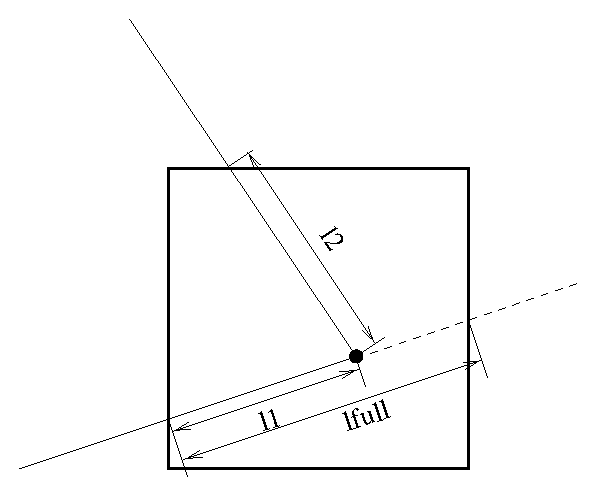
\includegraphics[width=0.6\textwidth]{figures/scatter.eps}
  \end{center}
\caption{The geometry of a scattering event within a powder sample.}
\label{powderFig}
\end{figure}

The probability for a neutron to be scattered from within the interval
$[ l_1 ; l_1+dl ]$ will be
\begin{equation}
\Pi(l_1) dl = \mu^s P(l_1) dl ,
\end{equation}
while the probability for a neutron to be scattered from within
this interval into the solid angle $\Omega$ {\em and}
not being scattered further
or absorbed on the way out of the sample is
\begin{equation}
\Pi(l_1,\Omega) dl d\Omega = 
  \mu^s P(l_1) P(l_2) \gamma(\Omega) d\Omega dl ,
\end{equation}
where $\gamma(\Omega)$ is the directional distribution
of the scattered neutrons, and $l_2$ is determined by $l_1$, 
$\Omega$, and the sample geometry, see figure \ref{powderFig}.

In our Monte-Carlo simulations, we will often choose the scattering
parameters by making a Monte-Carlo choice of $l_1$ and $\Omega$
from a distribution different from $\Pi(l_1,\Omega)$.
By doing this, we must adjust $\pi_i$ according to
the probability transformation rule (\ref{probrule}).
If we {\em e.g.}\ choose the scattering depth, $l_1$,
from a flat distribution in $[ 0 ; l_{\rm full} ]$, 
and choose the directional dependence from $g(\Omega)$,
we have a Monte Carlo probability
\begin{equation}
f(l_1,\Omega) = g(\Omega) / l_{\rm full} ,
\end{equation}
$l_{\rm full}$ is here the path length through the sample
as taken by a non-scattered neutron (although we here 
assume that all simulated neutrons are being scattered).
According to (\ref{probrule}), the neutron weight factor
is now adjusted by the amount
\begin{equation}     \label{sampleprob}
\pi_i(l_1,\Omega) =
 \mu^s l_{\rm full} \exp \left[ - (l_1+l_2) (\mu^a + \mu^s) \right]
  \frac{\gamma(\Omega)}{g(\Omega)} .
\end{equation}

In analogy with the source components, it is possible to define
interesting directions for the scattering.  
One will then try to focus the scattered neutrons,
choosing a $g(\Omega)$, which peaks around these directions. 
To do this, one uses (\ref{sampleprob}), where the
fraction $\gamma(\Omega)/g(\Omega)$ corrects for the focusing.
One must choose a proper distribution so that
$g(\Omega) > 0$ in every interesting direction. If this is not the 
case, the Monte Carlo simulation gives incorrect results.

All samples of the powder type have been constructed with a focusing
and a non-focusing option.

\subsection{V\_sample: An incoherent scatterer, the V-sample}
\label{s:v_sample}

A  vanadium sample is frequently being used for 
calibration purposes, as
almost all of the scattering from the sample occurs incoherently.

In the component {\bf V\_sample}, shown in \ref{c:v-sample}
we assume {\em only} absorption and incoherent scattering.
For the sample geometry, we have assumed the shape of a 
hollow cylinder (which has the solid cylinder as a limiting case).
The sample dimensions are: Inner radius $r_i$, 
outer radius $r_o$, and height $h$, see figure \ref{f:v-sample}.
\begin{figure}
  \begin{center}
    \psfrag{ri}{$r_i$}
    \psfrag{ro}{$r_o$}
    \psfrag{h}{$h$}
    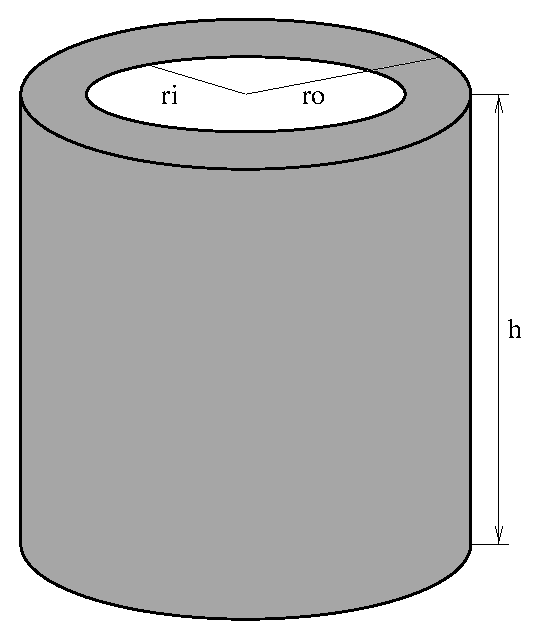
\includegraphics[width=0.3\textwidth]{figures/vsample.eps}
  \end{center}
\caption{The geometry of the hollow-cylinder vanadium sample.}
\label{f:v-sample}
\end{figure}

When calculating the neutron path length within
the sample material, the kernel function 
\verb+CYLINDER_INTERSECT+
is used twice, once for the outer radius and once 
for the inner radius.

The incoherent scattering gives
a completely uniform angular distribution of the scattered
neutrons from each V-nucleus: $\gamma(\Omega) = 1/4\pi$.
For the focusing we choose to have a uniform distribution on
a target sphere of radius $r_{\rm t}$, at the position 
$(x_{\rm t},y_{\rm t},z_{\rm t})$
in the local coordinate system.
This gives an angular distribution (in a small angle approximation)
of 
\begin{equation}
g(\Omega) = \frac{1}{4\pi} 
  \frac{x_{\rm t}^2+y_{\rm t}^2+z_{\rm t}^2}{(\pi r_{\rm t}^2)}.
\end{equation}

The input parameters for the component {\bf V\_sample} are
the sample dimensions ($r_i$, $r_o$, and $h$),
the packing factor for the V-sample (\verb+pack+),
and the focusing parameters ($x_{\rm t}, y_{\rm t}, z_{\rm t}$, 
and $r_{\rm t}$) for the target sphere. 
The relevant material parameters for V
($\sigma_c^s$, $\sigma_c^a$, and the unit cell volume $V_c$) 
are contained within the component.

Note: When simulating a realistic V-sample of this geometry
one finds that  the resulting direction dependence 
of the scattered intensity is {\em not} isotropic.
This is explained by the variation of attenuation with
scattering angle.
One test result is shown in Appendix \ref{testresults}.

\subsection{Powder1: A general powder sample}
\subsubsection{General considerations}
An ideal powder sample consists of many small
crystallites, although each crystallite is sufficiently
large not to cause size broadening.
The orientation of the crystallites is evenly distributed,
and there is thus always a certain number of
crystallites oriented to fulfill the Bragg condition
\begin{equation}   \label{Bragg}
n \lambda = 2 d \sin \theta ,
\end{equation}
where $n$ is the order of the scattering (an integer), $\lambda$
is the neutron wavelength, $d$ is the lattice spacing of the sample,
and $2 \theta$ is the scattering angle, see figure \ref{coneFig}.
As all crystal orientations
are realised in a powder sample, the neutrons are scattered within a
{\em Debye-Scherrer cone} of opening angle $4 \theta$ \cite{bacon}.

\begin{figure}
  \begin{center}
    \psfrag{2theta}[c][c]{$2\theta$}
    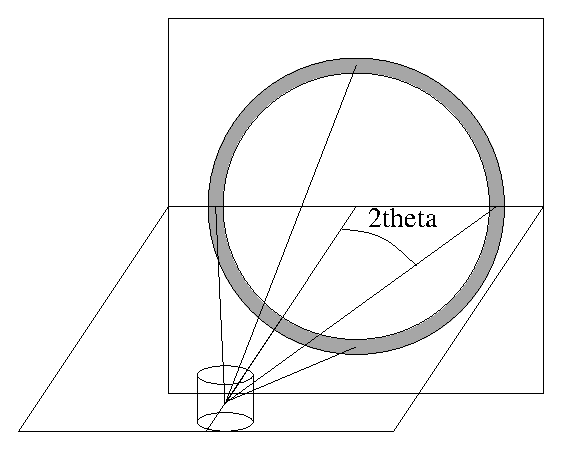
\includegraphics[width=0.6\textwidth]{figures/powder.eps}
  \end{center}
\caption{The scattering geometry of a powder sample showing the
Debye-Scherrer cone and the Debye-Scherrer circle.} 
\label{coneFig}
\end{figure}

Equation (\ref{Bragg}) may be cast into the form
\begin{equation}
|{\bf Q}| = 2 |{\bf k}| \sin \theta ,
\end{equation}
where {\bf Q} is a vector of the reciprocal lattice, and {\bf k} is
the wave vector of the neutron. It is seen that only
reciprocal vectors fulfilling $|{\bf Q}| < 2 |{\bf k}|$ 
contribute to the scattering.
For a complete treatment of the powder sample, one needs to take
into account all these {\bf Q}-values, since each of them contribute 
to the attenuation.

The textbook expression for the scattering intensity
from one reflection in a slab-shaped powder sample,
much larger than the beam cross section, reads \cite{bacon}
\begin{eqnarray}
\label{e:slab}
\frac{P}{P_0} &=& \frac{\lambda^3 l_s}{4\pi r} \frac{\rho'}{\rho}
         t j N_c^2 |F({\bf Q})|^2 \exp(-2W)
         \frac{\exp(-\mu^{\rm a} t / cos \theta)}{\sin^2(2\theta)} \\ 
|F({\bf Q})|^2 &=& 
 \left| \sum_j b_j \exp({\bf R}_j \cdot {\bf Q}) \right|^2 , 
\end{eqnarray}
where the sum in the structure factor runs over all atoms in one unit cell.
The meanings and units of the symbols are
%
\begin{quote}\begin{tabular}{ccl}
$P_0$ & s$^{-1}$ & Incoming intensity of neutrons \\
$P$   & s$^{-1}$ & Detected intensity of neutrons \\
$l_s$ & m        & Height of detector \\
$r$   & m        & Distance from sample to detector \\
$\rho'/\rho$ & 1 & Packing factor of the powder \\
$t$   & m        & Slab thickness \\
$j$   & 1        & Multiplicity of the reflection \\
$N_c$ & m$^{-3}$ & Density of unit cells in bulk material\\
$|F({\bf Q})|^2$ & m$^2$  & Structure factor \\
$\exp(-2W)$ & 1  & Debye-Waller factor \\
$\mu^a$ & m$^{-1}$ & Linear attenuation factor due to absorption. \\
\end{tabular}\end{quote}
%
In analogy with this, the textbook expression for a cylinder shaped powder
sample, completely illuminated by the beam, reads \cite{bacon}
\begin{equation}
\frac{P}{\Psi_0} = 
 \frac{V \rho'}{\rho} N_c^2 |F({\bf Q})|^2 j \exp(-2W)
                    \frac{A_{hkl}}{\sin(\theta)\sin(2\theta)}
                    \frac{l_s}{2\pi r} \frac{\lambda^3}{4} ,
\end{equation}
where the new symbols are
%
\begin{quote}\begin{tabular}{ccl}
$\Psi_0$  & s$^{-1}$m$^{-2}$ & Incoming beam flux \\
$V$       & m$^3$    & Sample volume \\
$A_{hkl}$ & 1        & Attenuation factor. \\
\end{tabular}\end{quote}
%
Eq.\ (\ref{e:slab}) for a slab shaped sample
may be cast into the form of the cylinder expression above
by using the substitutions
%
\begin{quote}\begin{tabular}{lrcl}
Incoming flux & $P_0 / (w h \cos\theta)$ & $\rightarrow$ & $\Psi_0$ \\
Sample volume & $w h t$ & $\rightarrow$ & $V$ \\
Absorption factor & $\exp(-\mu^a t / \cos\theta)$ & $\rightarrow$ & $A_{hkl}$, \\
\end{tabular}\end{quote}
%
where $h$ and $w$ are the height and width of the sample, respectively.
Often, one defines the {\em scattering power} as
\begin{equation}
Q \equiv N^2 \frac{|F({\bf Q})|^2 \lambda^3}{V \sin(2\theta)}
 = N_c^2 V \frac{\rho'}{\rho} \frac{|F({\bf Q})|^2 \lambda^3}{\sin(2\theta)} ,
\end{equation}
where $N$ is the number of unit cells.

A cut though the Debye-Scherrer cone perpendicular to its axis
is a circle. At the distance $r$ from the sample, the radius of this
circle is $r \sin(2\theta)$. Thus, the detector (in a small angle
approximation) only counts a fraction $f_d = l_s / (2 \pi r \sin(2 \theta))$
of the scattered neutrons.
One may now calculate the
linear attenuation coefficient in the material due to scattering
(from one {\bf Q}-value only):
\begin{equation}
\label{e:attenu}
\mu^s \equiv -\frac{1}{P_0} \frac{d(P/f_d)}{dl}
  = \frac{Q}{V} j \exp(-2W) \cos(\theta) .
\end{equation}
A powder sample will in general have several allowed reflections 
${\bf Q}_j$, which will all contribute to the attenuation. 
These reflections will have different values of 
$|F({\bf Q}_j)|^2$ (and hence of $Q_j$), $j_j$, $\exp(-2W_j)$, 
and $\theta_j$.
The total attenuation through the sample due to scattering is given by
$\mu^s = \mu_{\rm inc}^s + \sum_j \mu^s_j $, 
where $\mu_{\rm inc}^s$ represents the incoherent scattering.

\subsubsection{This implementation}
For component {\bf Powder1}, we assume that the sample 
has the shape of a solid cylinder. 
Further, the incoherent scattering is only taken into account
by the attenuation of the beam, given by (\ref{e:attenu}) 
and $\sigma_c^a$.
The incoherently scattered neutrons are not
propagated through to the detector, but rather not generated at all.
Focusing is performed by only scattering into one angular
interval, $d\phi$ of the Debye-Scherrer circle. The center of this
interval is located at the point where the Debye-Scherrer circle
intersects the half-plane defined by the initial velocity, ${\bf v}_{\rm i}$,
and a user-specified vector, {\bf f}. 
Multiple scattering is not implemented.

The input parameters for this component are
%
\begin{quote}\begin{tabular}{ccl}
$r$ & m & Radius of cylinder \\
$h$ & m & Height of cylinder \\
$\sigma_c^a$ & fm$^2$ & Absorption cross section per unit cell (at 2200 m/s) \\
$\sigma_{i,c}^s$ & (fm)$^2$ & Incoherent scattering cross section per unit cell \\
$\rho'/\rho$ & 1 & Packing factor \\
$V_c$ & \AA$^3$ & Volume of unit cell \\
${\bf Q}$ & \AA$^{-1}$ & The reciprocal lattice vector under consideration \\
$|F({\bf Q}_j)|^2$ & (fm)$^2$ &
 Structure factor \\
$j$ & 1 & Multiplicity of reflection \\
$\exp(-2W)$ & 1 & Debye-Waller factor \\
$d\phi$ & deg & Angular interval of focusing \\ 
$f_x$ & m & \\
$f_y$ & m & Focusing vector\\
$f_z$ & m & \\
\end{tabular}\end{quote}
%
The source text for the component is shown in Appendix
\ref{c:powder1}.

In a later version, more reciprocal lattice vectors will be
allowed. Further, we intent to include the effect of multiple
scattering.


% Emacs settings: -*-mode: latex; TeX-master: "manual.tex"; -*-

\chapter{Inelastic scattering kernels}
\label{s:inelastic}

In this section, samples with inelastic scattering are
described. Currently, only a single sample is available that scatters
uniformly in $({\bf Q}, \omega)$ and is used for computing resolution
functions in tripple-axis instruments.

\section{Res\_sample: A uniform scatterer for resolution calculation}
\label{s:res_sample}

The component \textbf{Res\_sample} models an inelastic sample that
scatters completely homogeneous in position and energy; regardless of
the state of the incoming neutron, all directions and energies for the
scattered neutron have the same probability. This clearly does not
correspond any physically realizable samples, but the component is very
useful for computation of the resolution function and may also be used
for test and debugging purposes. The component is designed to be used
together with the \textbf{Res\_monitor} component, described in
section~\ref{s:res_monitor}.

The shape of the sample is either a hollow cylinder (like the vanadium
sample described in section~\ref{s:v_sample}) or a rectangular box. The
hollow cylinder shape is specified with inner and outer radius \textit{radius\_i}
and \textit{radius\_o} and height \textit{h}. If \textit{radius\_o} is
negative, the shape is instead a box of width \textit{radius\_i} along
the X axis, height \textit{h}, and thickness $-\textit{radius\_o}$ along the
Z axis, centered on the Z axis and with the front face in the X-Y
plane. See figure~\ref{f:res_sample}.\par
%
\begin{figure}[htbp]
  \begin{center}
        \psfrag{ri}[c][c]{\textit{radius\_i}}
        \psfrag{ro}[c][c]{\textit{radius\_o}}
        \psfrag{h}[c][c]{\textit{h}}
        \psfrag{bri}[c][c]{\textit{radius\_i}}
        \psfrag{bro}[c][c]{$-\textit{radius\_o}$}
        \psfrag{bh}[c][c]{\textit{h}}
        \psfrag{X}[c][c]{\textit{X}}
        \psfrag{Y}[c][c]{\textit{Y}}
        \psfrag{Z}[c][c]{\textit{Z}}
        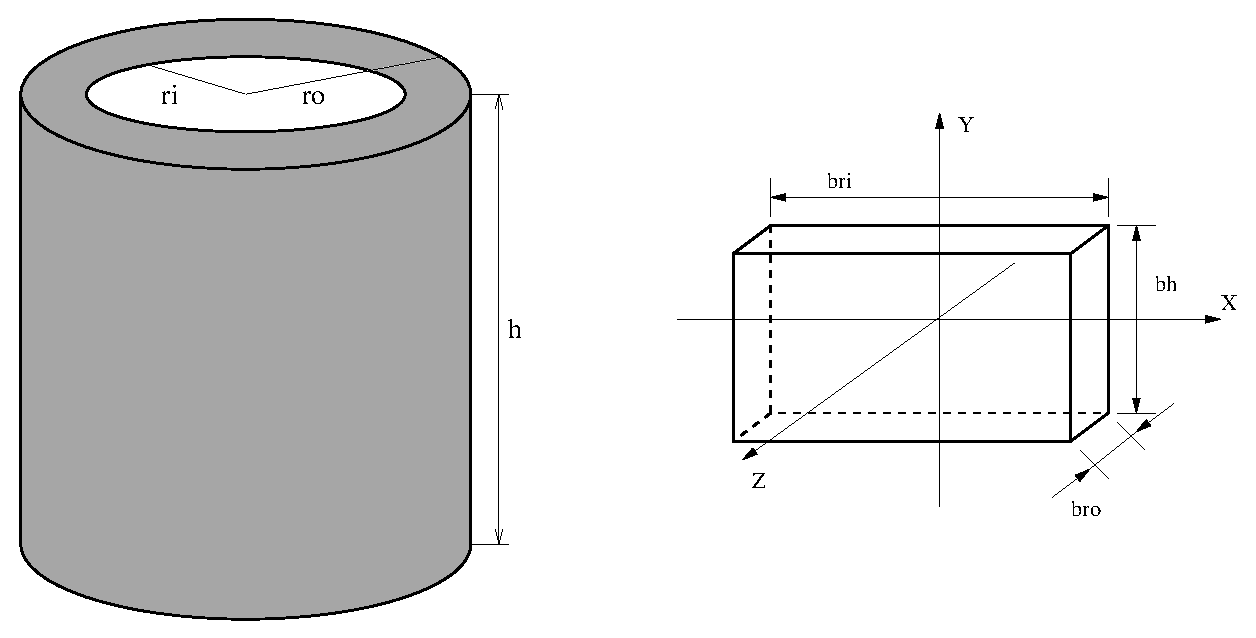
\includegraphics[width=0.9\textwidth]{figures/res_sample.eps}
    \caption{The two possible shapes of the \textbf{Res\_sample} component.}
    \label{f:res_sample}
  \end{center}
\end{figure}
%
The component only propagates the neutrons that are scattered; neutrons
that would pass through or miss the sample are absorbed. There is no
modeling of the cross section of the sample, secondary extinction
\textit{etc.}; the scattering probability is proportional to the neutron
flight path length inside the sample, with the constant of
proportionality arbitrarily set to $1/(2|\textit{radius\_o}|)$. The
reason for this is that the component is designed for computing the resolution
function of an instrument, including the sample size but independent of
any sample properties such as scattering and absorbtion cross sections.

The point of scattering in the sample is chosen at a random position
along the neutron flight path inside the sample, and the scattered
neutron is given a random energy and direction. The energy is selected in
a user-specified interval $[E_0-\Delta E; E_0+\Delta E]$ which must be
chosen large enough to cover all interesting neutrons, but preferably
not excessively large for reasons of efficiency. Similarly, the
direction is chosen in a user-specified range; the range is such that a
sphere of given center and radius is fully illuminated.

A special feature, used when computing resolution functions, is that the
component stores complete information about the scattering event in the
output parameter \textit{res\_struct}. The information includes initial
and final wave vectors, the coordinates of the scattering point, and the
neutron weight after the scattering event. From this information the
scattering parameters $({\bf Q}_i, \omega_i)$ for every scattering event
$i$ may be recorded and used to compute the resolution function of an
instrument, as explained below. For an example of how to use the
information in the output parameter, see the description of the
\textbf{Res\_monitor} component in section~\ref{s:res_monitor}.

The input parameters to the \textbf{Res\_sample} components are the
sample dimensions \textit{radius\_i}, \textit{radius\_o}, and
\textit{h}, all in meters; the center of the scattered energy range
\textit{E0} and the energy spread \textit{dE} in meV; and the target
sphere position in the local coordinate system \textit{target\_x},
\textit{target\_y}, \textit{target\_z}, and radius \textit{focus\_r}, in
meters. The only output parameter is \textit{res\_struct} containing
information about the scattering event, with all vectors given in the
local coordinate system of the component in units of meter.

\subsection{Background}

In an experiment, as well as in the simulation, the expected intensity
is by definition of the resolution function given by
%
$$
  I = \int R({\bf Q}, \omega) \sigma({\bf Q}, \omega) d{\bf Q}d\omega
$$
%
Here $I({\bf Q}_0, \omega_0)$ is the measured or simulated intensity in
the detector, $R$ is the resolution function for the instrument in a
given setup, $\sigma$ is the scattering cross section of the sample, and
$({\bf Q}, \omega)$ denote the scattering vector and energy transfer in
the sample. For the uniform scatterer, $\sigma({\bf Q}, \omega) = 1/V_0$
is a constant, so we have
%
$$
  I = 1/V_0 \int R({\bf Q}, \omega) d{\bf Q}d\omega
$$
%
If we instead consider only the intensity contributed by scattering with
parameters $({\bf Q}, \omega)$ that lie within a small part $\Delta\Omega$ of
the total phase space and has volume $\Delta V$,
%
$$
  I_{\Delta\Omega} = 1/V_0 \int_{\Delta\Omega} R({\bf Q}, \omega) d{\bf Q}d\omega
  = \frac{\Delta V}{V_0} R(\Delta\Omega)
$$
%
(where $R(\Delta\Omega)$ denotes the average value of $R$ over
$\Delta\Omega$), we get a good approximation of the value of $R$
provided that $\Delta\Omega$ is sufficiently small. This is useful with
the output from the simulations, since $I_{\Delta\Omega}$ is
approximated by

$$ I_{\Delta\Omega} \approx \sum_{({\bf Q_i},\omega_i) \in \Delta\Omega} p_i $$


This can be used to
histogram the resolution function or visualize it in different ways. The
3D visualization of the resolution function produced by the
\verb+mcresplot+ program for example uses this by displaying a cloud of
dots, the local density of which is proportional to the resolution
function.

The \verb+mcresplot+ program also computes the covariance and resolution
matrices. Letting $(x^1_i,x^2_i,x^3_i,x^4_i)$ denote the $({\bf
  Q_i},\omega_i)$ values obtained from the scattering events in the
simulation and $\mu^j = (\sum_i p_i x^j_i) / (\sum_i p_i)$ the mean
value of $x^j_i$, the covariance matrix is computed as
$$ {\bf C}_{jk} = \Big(\sum_i p_i (x^j_i - \mu_j) (x^k_i - \mu_k)\Big) /
   \Big(\sum_i p_i\Big) $$
This covariance matrix is given in the local coordinate system of the
sample component. The \verb+mcresplot+ program actually outputs the
covariance matrix in another coordinate system which is rotated around
the Y axis so that the projection to the X-Z plane of the average
scattering vector ${\bf Q}_{\rm avg} = (\sum_i p_i {\bf Q}_i) / (\sum_i
p_i)$ is parallel to the X axis.

The resolution matrix ${\bf M}$ is the inverse of the covariance matrix
and is also output in the rotated coordinate system by \verb+mcresplot+.
The 4-dimensional gaussian distribution, defined by
\begin{equation}
  \label{eq:gauss-res}
  f({\bf X}) = e^{-\frac{1}{2}{\bf X}^T {\bf M} {\bf X}}
\end{equation}
where ${\bf X} = ({\bf Q},\omega)$, has covariance matrix ${\bf C}$ and
thus defines the gaussian resolution function with the same covariance
as the resolution computed by the simulation.

The \verb+mcresplot+ program provides for the simultaneous visualization
of the computed and the gaussian resolution function by obtaining an
appropriate number of random points with the statistical
distribution~(\ref{eq:gauss-res}). Each point ${\bf X}$ is obtained as
follows: A vector ${\bf Y}$ is generated of four individually gaussian
distributed random numbers with mean zero and variance one. Using the
Cholesky decomposition of ${\bf C}$, ${\bf C} = {\bf L}{\bf L}^T$, we
have
$$ {\bf X} = {\bf L} {\bf Y}.$$




